\documentclass{article}
\usepackage{float}
\usepackage[utf8]{inputenc}
\usepackage[table,xcdraw]{xcolor} 
\usepackage{soul} 
\usepackage{graphicx}
\usepackage{tabularx} % Aggiunto per far funzionare la tabella larga
\usepackage{makecell}
\usepackage{multirow}
\usepackage[hidelinks]{hyperref}
\usepackage{svg}

\begin{document}

\begin{titlepage}
    \centering
    
    % Logo
    
\includegraphics[width=0.5\textwidth]{Logo.jpg}
    \vspace{0.5cm}
    
    % Università e corso
    {\large Università degli Studi di Napoli Federico II}\\
    \vspace{0.2cm}
    {\large Corso di Ingegneria del Software}\\
    
    \vspace{2cm}
    
    % Titolo
    {\Huge \textbf{DietiEstates25}}\\
    \vspace{0.3cm}
    {\large Documentazione del Progetto}
    
    \vspace{2cm}
    
    % Studenti e docenti affiancati
    \begin{minipage}{0.45\textwidth}
        \raggedright
        \textbf{Studenti:}\\
        Pietro\\
        Gino
    \end{minipage}
    \hfill
    \begin{minipage}{0.45\textwidth}
        \raggedleft
        \textbf{Docenti:}\\
       Prof. Sergio DI MARTINO\\
       Prof. Luigi Libero Lucio STARACE
    \end{minipage}
    
    \vfill

\end{titlepage}

\newpage
\tableofcontents
\newpage
\section{Documento dei Requisiti Software}

Il presente documento definisce i requisiti software attraverso una formalizzazione strutturata. L'obiettivo è delineare le funzionalità del sistema e il dominio applicativo in modo univoco, eliminando ogni ambiguità interpretativa grazie all'uso di notazioni complementari.

\subsection{Glossario}

Il Glossario è una raccolta di vocaboli specifici del dominio applicativo, accompagnati dalla spiegazione del loro significato nel contesto del sistema. Questa sezione mira a superare le barriere comunicative tra stakeholder e sviluppatori.

\renewcommand{\arraystretch}{1.5} % Rende le righe più alte e leggibili
\begin{table}[h]
\centering
\begin{tabularx}{\textwidth}{|l|X|}
\hline
\rowcolor[HTML]{010066} 
{\color[HTML]{EFEFEF} \textit{\textbf{Nome}}} & {\color[HTML]{FFFFFF} \textit{\textbf{Descrizione}}} \\ \hline
Amministratore agenzia & Utente con pieni poteri di gestione su organico e configurazioni di sistema. \\ \hline
Supporto               & Profilo tecnico per la manutenzione e l'assistenza operativa diretta. \\ \hline
Agente immobiliare     & Operatore che gestisce il portafoglio immobili e la relazione con i clienti. \\ \hline
Cliente                & Utente registrato che interagisce per acquisto, vendita o affitto di immobili. \\ \hline
Cliente non registrato & Visitatore che consulta pubblicamente gli annunci senza autenticazione. \\ \hline
Immobile               & Entità fisica e catastale oggetto dell'attività di intermediazione. \\ \hline
\end{tabularx}
\end{table}

\newpage
\subsection{Casi D'uso}
In questa sezione vengono presentati i principali casi d’uso del sistema Dieti-Estates25. Attraverso i diagrammi dei casi d'uso è possibile visualizzare le funzionalità del sistema dal punto di vista degli utenti, rappresentando graficamente gli attori che interagiscono con la piattaforma, i casi d'uso (ovvero le azioni necessarie per raggiungere uno specifico obiettivo) e le loro relazioni

\newpage
\begin{figure}[H]
    \centering
    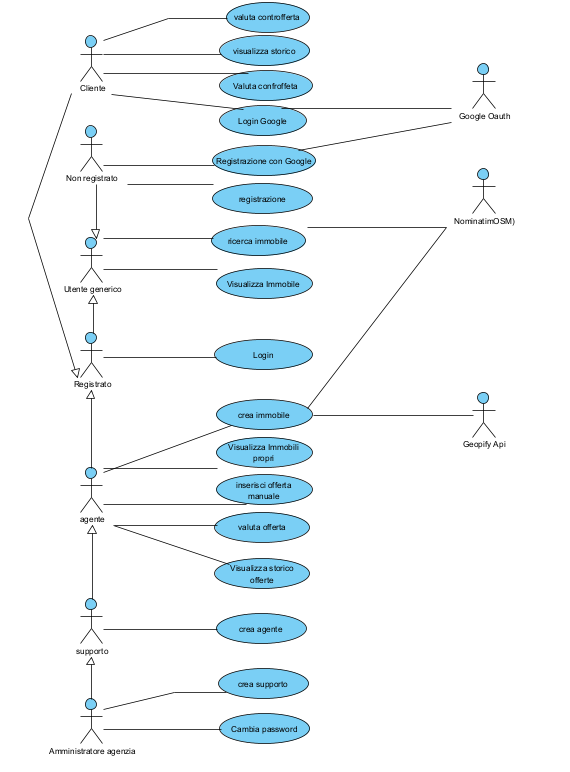
\includegraphics[width=\textwidth]{Usecase0.png}
    \caption{Diagramma dei casi d'uso -- DietiEstates25}
\end{figure}
\newpage
\subsection{Personas}
Le user personas sono strumenti chiave della strategia di sviluppo di un prodotto digitale, che consentono di creare una rappresentazione dettagliata e accurata dei diversi tipi di utenti che interagiscono con un brand.
Ogni user persona è caratterizzato da un nome, una foto e una descrizione dettagliata delle sue caratteristiche, dei suoi obiettivi, delle sue sfide e dei suoi bisogni, nell’ambito in cui opera l’azienda.

\subsubsection{Personas 1: Cliente in cerca di una casa in affitto}
\noindent % Fondamentale per allineare a sinistra
\begin{minipage}[c]{0.4\textwidth} 
    \centering
    
\includegraphics[width=\textwidth]{Cliente.png} 
\end{minipage}% <--- IL SIMBOLO % QUI È FONDAMENTALE (rimuove lo spazio fantasma)
\hfill 
\begin{minipage}[c]{0.55\textwidth} 
    \begin{itemize}
        \item \textbf{Nome:} Marco Rovere
        \item \textbf{Età:} 26 anni
        \item \textbf{Occupazione:} Sviluppatore
    \end{itemize}
\end{minipage}

\begin{itemize}
    \item \textbf{Descrizione:} Marco è un giovane sviluppatore che si è trasferito 
    in una nuova città per lavoro e cerca un appartamento in affitto 
    comodo e ben collegato. Abituato a usare strumenti digitali, 
    vuole trovare casa in modo rapido e autonomo, senza dover 
    contattare agenzie fisicamente.
    
    \item \textbf{Obiettivo:} Trovare l'immobile ideale senza stress, potendo 
    navigare tra gli annunci in modo semplice e intuitivo, filtrare 
    i risultati in base alle proprie esigenze e visualizzare tutte 
    le informazioni necessarie in un unico posto, senza dover 
    perdere tempo a contattare più agenzie o visitare siti diversi.
\end{itemize}

\vspace{1 em}
\subsubsection{Personas 2: Agente Immobiliare professionista}
\noindent 
\begin{minipage}[c]{0.4\textwidth} 
    \centering
    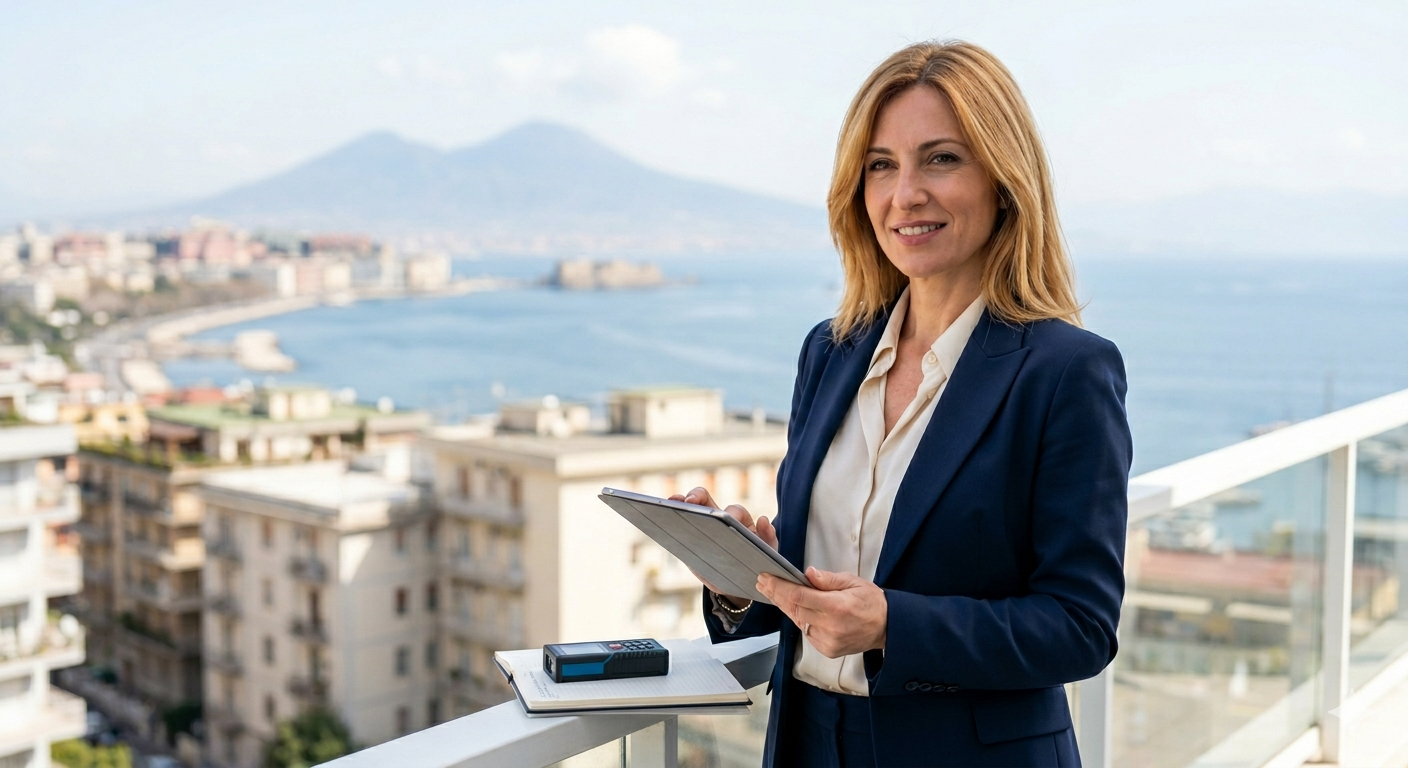
\includegraphics[width=\textwidth]{Agente.png} 
\end{minipage}%
\hfill 
\begin{minipage}[c]{0.55\textwidth} 
    \begin{itemize}
        \item \textbf{Nome:} Elena Visconti
        \item \textbf{Età:} 42 anni
        \item \textbf{Occupazione:} Agente Immobiliare Senior
    \end{itemize}
\end{minipage}

\begin{itemize}
    \item \textbf{Descrizione:} Elena lavora nel settore da oltre dieci anni. 
    La sua necessità principale è la mobilità: deve poter aggiornare lo stato 
    di un annuncio o caricare nuove foto direttamente dal suo tablet mentre 
    si trova sul luogo del sopralluogo, riducendo i tempi di inserimento 
    dati in ufficio.

    \item \textbf{Obiettivo:} Gestire i propri annunci in modo rapido e 
    flessibile, potendo operare direttamente dal campo senza dover 
    tornare in ufficio per ogni aggiornamento.
\end{itemize}

\subsubsection{Personas 3: Amministratore Agenzia}
\noindent 
\begin{minipage}[c]{0.4\textwidth} 
    \centering
    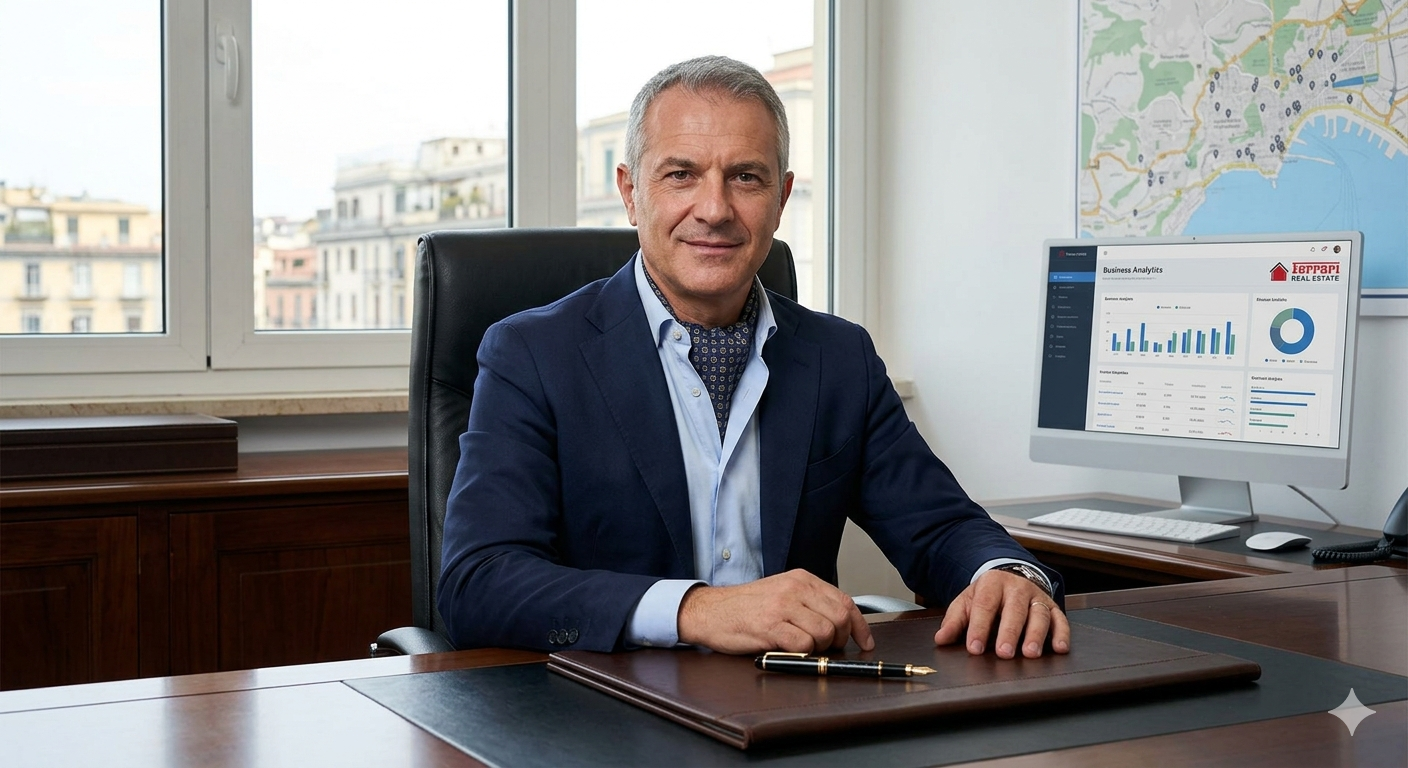
\includegraphics[width=\textwidth]{Amministratore.png} 
\end{minipage}%
\hfill 
\begin{minipage}[c]{0.55\textwidth} 
    \begin{itemize}
        \item \textbf{Nome:} Marco Rinaldi
        \item \textbf{Età:} 50 anni
        \item \textbf{Occupazione:} Titolare Agenzia Immobiliare
    \end{itemize}
\end{minipage}

\begin{itemize}
    \item \textbf{Descrizione:} Marco è il titolare di un'agenzia immobiliare e si occupa della gestione complessiva del business. Il suo interesse principale è avere una visione chiara e aggiornata delle attività: monitorare le performance degli agenti, controllare lo stato degli immobili e analizzare i dati di vendita. Predilige strumenti che offrano dashboard intuitive e report dettagliati per supportare decisioni strategiche rapide ed efficaci.

\item \textbf{Obiettivo:} Avere il pieno controllo sulla propria agenzia, 
utilizzare la piattaforma in modo semplice e intuitivo e aumentare 
la visibilità della sua agenzia.
\end{itemize}


\newpage
\subsection{Formalizzazione dei casi d'uso}
Per rappresentare le funzionalità del sistema in modo strutturato, viene utilizzato 
il diagramma dei Use case diagram, uno strumento UML che permette 
di descrivere cosa il sistema fa dal punto di vista degli utenti. Nel diagramma 
sono identificati gli attori che interagiscono con il sistema e le operazioni 
che ciascuno di essi può compiere.

\newpage
\begin{table}[htbp]
\centering
\renewcommand{\arraystretch}{1.5}
\begin{tabular}{|p{3cm}|l|p{4.5cm}|p{4.5cm}|}
\hline
\rowcolor[HTML]{010066} 
{\color[HTML]{EFEFEF} \textbf{Caso d'uso \#01}} & \multicolumn{3}{l|}{\color[HTML]{FFFFFF} \textbf{Crea account supporto}} \\ \hline

\textbf{Scopo} & \multicolumn{3}{l|}{Creare un nuovo account supporto.} \\ \hline

\textbf{Precondizioni} & \multicolumn{3}{l|}{utente autenticato come amministratore e visualizza la dashboard.} \\ \hline

\textbf{Condizione Successo} & \multicolumn{3}{l|}{Creazione del supporto.} \\ \hline

\textbf{Condizione Fallimento} & \multicolumn{3}{l|}{Nessuna registrazione effettuata.} \\ \hline

\textbf{Attore principale} & \multicolumn{3}{l|}{Amministratore dell'agenzia.} \\ \hline

\textbf{Trigger} & \multicolumn{3}{l|}{Click su ``Crea Admin'' (UC01\_M01).} \\ \hline

\hline
% La cella "Scenario Principale" raggruppa le 6 righe successive
\multirow{6}{3cm}{\textbf{Scenario Principale}} 
   & \textbf{Passo} & \textbf{Amministratore dell'agenzia} & \textbf{Sistema} \\ \cline{2-4}
   & 01 & Clicca ``Crea Supporto'' & \\ \cline{2-4}
   & 02 & & Mostra UC01\_M02 \\ \cline{2-4}
   & 03 & Compila il modulo & \\ \cline{2-4}
   & 04 & & Mostra UC01\_M03 \\ \cline{2-4}
   & 05 & Clicca sul bottone di invio & \\ \cline{2-4}
   & 06 & & caso d'uso terminato con successo \\ \hline
% --- ESTENSIONE #1 ---
\multirow{4}{3cm}{\textbf{Estensione \#1}} 
   & \textbf{Passo} & \textbf{Proprietario} & \textbf{Sistema} \\ \cline{2-4}
   & 3.1 & inserisce nel form email già esistente & \\ \cline{2-4}
   & 3.2 & clicca bottone di invio &  \\ \hline
   & 3.3 & & messaggio email già esistente \\ \hline
\multirow{3}{3cm}{\textbf{Estensione \#2}} 
   & \textbf{Passo} & \textbf{Proprietario} & \textbf{Sistema} \\ \cline{2-4}
   & 3.1 & Clicca su uno dei bottoni \newline cliccabili nella barra di navigazione
 & \\ \cline{2-4}
   & 3.2 & & Termina il caso d’uso \\ \hline
   \multirow{3}{3cm}{\textbf{Estensione \#3}} 
   & \textbf{Passo} & \textbf{Proprietario} & \textbf{Sistema} \\ \cline{2-4}
   & 3.3 & clicca su annulla & \\ \cline{2-4}
   & 4.3 & & torna alla dashboard \\ \hline
   
\end{tabular}

\caption{Tabella di Cockburn - UC01}
\end{table}



\begin{table}[H]
\centering
\renewcommand{\arraystretch}{1.5}
\begin{tabular}{|p{3cm}|l|p{4.5cm}|p{4.5cm}|}
\hline
\rowcolor[HTML]{010066} 
{\color[HTML]{EFEFEF} \textbf{Caso d'uso \#02}} & \multicolumn{3}{l|}{\color[HTML]{FFFFFF} \textbf{Crea account Agente}} \\ \hline

\textbf{Scopo} & \multicolumn{3}{l|}{Creare un nuovo agente immobiliare.} \\ \hline

\textbf{Precondizioni} & \multicolumn{3}{l|}{L'utente Supporto deve aver eseguito il login.} \\ \hline

\textbf{Condizione Successo} & \multicolumn{3}{l|}{Account Agente registrato e credenziali inviate via e-mail.} \\ \hline

\textbf{Condizione Fallimento} & \multicolumn{3}{l|}{L'account non viene creato.} \\ \hline

\textbf{Attore principale} & \multicolumn{3}{l|}{Personale di Supporto.} \\ \hline

\textbf{Trigger} & \multicolumn{3}{l|}{Click su ``Nuovo Agente'' (UC02\_M01).} \\ \hline

\hline
% --- SCENARIO PRINCIPALE ---
\multirow{6}{3cm}{\textbf{Scenario Principale}} 
   & \textbf{Passo} & \textbf{Supporto} & \textbf{Sistema} \\ \cline{2-4}
   & 01 & Clicca ``Nuovo Agente'' & \\ \cline{2-4}
   & 02 & & Mostra modulo creazione UC02\_M02 \\ \cline{2-4}
   & 03 & Inserisce dati agente & \\ \cline{2-4}
   & 04 & & Valida dati e mostra UC02\_M03 \\ \cline{2-4}
   & 05 & Conferma creazione & \\ \cline{2-4}
   & 06 & & Invia e-mail e termina caso d'uso \\ \hline

\hline
\multirow{3}{3cm}{\textbf{Estensione \#1}} 
   & \textbf{Passo} & \textbf{Proprietario} & \textbf{Sistema} \\ \cline{2-4}
   & 3.1 & inserisce Email già esistente & \\ \cline{2-4}
   & 3.2 & clicca bottone per creare & \\ \cline{2-4}
   & 3.3 & & Mostra errore \\ \hline
   \multirow{3}{3cm}{\textbf{Estensione \#1}} 
   & \textbf{Passo} & \textbf{Proprietario} & \textbf{Sistema} \\ \cline{2-4}
   & 3.1 & clicca su annulla & \\ \cline{2-4}
   & 3.3 & & ritorna alla dasbaord \\ \hline
\multirow{3}{3cm}{\textbf{Estensione \#2}} 
   & \textbf{Passo} & \textbf{Proprietario} & \textbf{Sistema} \\ \cline{2-4}
   & 3.1 & Clicca su uno dei bottoni \newline cliccabili nella barra di navigazione
 & \\ \cline{2-4}
   & 3.2 & & Termina il caso d’uso \\ \hline
\end{tabular}
\caption{Tabella di Cockburn - UC02: Creazione Agente}
\end{table}
\clearpage






\begin{table}[H]
\centering
\renewcommand{\arraystretch}{1.5}
\begin{tabular}{|p{3cm}|l|p{4.5cm}|p{4.5cm}|}
\hline
\rowcolor[HTML]{010066} 
{\color[HTML]{EFEFEF} \textbf{Caso d'uso \#03}} & \multicolumn{3}{l|}{\color[HTML]{FFFFFF} \textbf{Inserimento Offerta Manuale}} \\ \hline

\textbf{Scopo} & \multicolumn{3}{l|}{Inserire un'offerta manualmente nel sistema.} \\ \hline

\textbf{Precondizioni} & \multicolumn{3}{l|}{Agente autenticato, sezione "I miei immobili".} \\ \hline

\textbf{Condizione Successo} & \multicolumn{3}{l|}{Offerta inserita correttamente nel sistema.} \\ \hline

\textbf{Condizione Fallimento} & \multicolumn{3}{l|}{Offerta non inserita.} \\ \hline

\textbf{Attore principale} & \multicolumn{3}{l|}{Agente.} \\ \hline

\textbf{Trigger} & \multicolumn{3}{l|}{Click su inserimento offerta manuale.} \\ \hline

\hline
% --- SCENARIO PRINCIPALE ---
\multirow{6}{3cm}{\textbf{Scenario Principale}} 
   & \textbf{Passo} & \textbf{Agente} & \textbf{Sistema} \\ \cline{2-4}
   & 01 & Seleziona la scritta di inserimento manuale & \\ \cline{2-4}
   & 02 & & Mostra modulo inserimento \\ \cline{2-4}
   & 03 & Inserisce i dati dell'offerta & \\ \cline{2-4}
   & 04 & & Valida i dati inseriti \\ \cline{2-4}
   & 05 & Clicca sul bottone per creare & \\ \cline{2-4}
   & 06 & & mostra messaggio ed è indirizzato allo storico \\ \hline

\hline
% --- ESTENSIONE #1 ---
\multirow{3}{3cm}{\textbf{Estensione \#1}} 
   & \textbf{Passo} & \textbf{Proprietario} & \textbf{Sistema} \\ \cline{2-4}
   & 3.1 & clicca sulla navbar & \\ \cline{2-4}
   & 3.3 & & fine use case \\ \hline

\end{tabular}
\caption{Tabella di Cockburn - UC03: Offerta Manuale}
\end{table}

\clearpage














\begin{table}[H]
\centering
\renewcommand{\arraystretch}{1.5}
\begin{tabular}{|p{2.8cm}|p{0.8cm}|p{4.2cm}|p{4.2cm}|}
\hline
\rowcolor[HTML]{010066} 
{\color[HTML]{EFEFEF} \textbf{Caso d'uso \#04}} & \multicolumn{3}{l|}{\color[HTML]{FFFFFF} \textbf{Visualizza Immobile}} \\ \hline
\textbf{Scopo} & \multicolumn{3}{l|}{Un utente generico vuole visualizzare un immobile con i suoi dettagli.} \\ \hline
\textbf{Precondizioni} & \multicolumn{3}{l|}{L'utente ha completato con successo il caso d'uso Ricerca Immobile.} \\ \hline
\textbf{Condizione Successo} & \multicolumn{3}{l|}{Il sistema carica tutte le informazioni dettagliate riguardo l'immobile.} \\ \hline
\textbf{Condizione Fallimento} & \multicolumn{3}{l|}{Il sistema non carica le informazioni dettagliate riguardo l'immobile.} \\ \hline
\textbf{Attore principale} & \multicolumn{3}{l|}{Utente generico.} \\ \hline
\textbf{Trigger} & \multicolumn{3}{l|}{Click su un immobile nella schermata UC04\_M01.} \\ \hline

% --- SCENARIO PRINCIPALE ---
\multirow{4}{2.8cm}{\textbf{Scenario Principale}} 
   & \textbf{Passo} & \textbf{Utente} & \textbf{Sistema} \\ \cline{2-4}
   & 01 & Clicca su un immobile & \\ \cline{2-4}
   & 02 & & Carica e mostra i dettagli dell'immobile \\ \cline{2-4}
   & 03 & & Termina caso d'uso \\ \hline

\end{tabular}
\caption{Tabella di Cockburn - UC04: Visualizza Immobile}
\end{table}

\clearpage

\newpage

\subsection{Requisiti non funzionali e di Dominio}
\subsubsection{Requisiti non funzionali}
I Requisiti Non-Funzionali descrivono vincoli sui servizi offerti dal
sistema, e sullo stesso processo di sviluppo


\begin{table}[h]
\centering
\begin{tabularx}{\textwidth}{|l|X|}
\hline
\rowcolor[HTML]{010066} 
{\color[HTML]{EFEFEF} \textit{\textbf{Nome}}} & {\color[HTML]{FFFFFF} \textit{\textit{Descrizione}}} \\ \hline
NFR01  &Il sistema deve essere implementato utilizzando linguaggi di programmazione 
Object-Oriented. \\ \hline
NFR02  & Le ricerche devono essere eseguite in meno di 6 secondi. \\ \hline
NFR03 &Il caricamento delle pagine deve essere inferiore a 3 secondi.  \\ \hline
NFR04 & Tutte le password devono essere salvate in modo sicuro \\ \hline
NFR05 & Il sistema dovrebbe essere operativo e accessibile il 99.9\% del tempo. \\ \hline
NFR06 & Supporto di almeno 100 utenti simultanei.\\ \hline
NFR07 & l’interfaccia deve essere semplice e facilmente utilizzabile da tutti gli utenti.\\ \hline

\end{tabularx}
\end{table}
\subsubsection{Requisiti di Dominio}

\begin{table}[h]
\centering
\begin{tabularx}{\textwidth}{|l|X|}
\hline
\rowcolor[HTML]{010066} 
{\color[HTML]{EFEFEF} \textit{\textbf{Nome}}} & {\color[HTML]{FFFFFF} \textit{\textit{Descrizione}}} \\ \hline
DR01  &Solo le agenzie immobiliari regolarmente registrate possono creare account per 
agenti immobiliari nel sistema.  \\ \hline
DR02  &Categorie obbligatorie "vendita" / "affitto".  \\ \hline
DR03  &Agenti gestiscono solo gli immobili di loro competenza.  \\ \hline
DR04  &Geocodifica tramite API esterne, precisione a livello civico.  \\ \hline

\end{tabularx}
\end{table}

\newpage
\section{Documento di Design del sistema}
\subsection{Architettura}

L'architettura utilizzata si compone di tre livelli:

\begin{itemize}
    \item \textbf{Frontend:} responsabile dell’interazione con l’utente.
    \item \textbf{Backend:} un’applicazione server-side che espone un set di API REST per la gestione dei dati e la logica di business.
    \item \textbf{Database:} sistema di persistenza dei dati relazionale.
\end{itemize}

L'architettura adottata garantisce una netta separazione delle responsabilità (Separation of Concerns). Poiché ogni componente è isolato e svolge un compito specifico, il sistema risulta intrinsecamente più scalabile e facile da manutenere.
\clearpage
\subsection{Tecnologie adottate}
Nella seguente sezione sono state raccolte le tecnologie usate per lo sviluppo del front-end e back-end. 
Inoltre si fa presente che un'altra tecnologia utilizzata sono le api di Google per l'autenticazione. 

Nelle seguenti tabelle sono elencate le tecnologie e le motivazioni. 


\begin{table}[htbp]
\centering
\caption{Tecnologie utilizzate per il Front-end} % Nome della tabella richiesto
\vspace{0.5em}
\renewcommand{\arraystretch}{1.5}
\begin{tabularx}{\textwidth}{|l|l|X|}
\hline
\rowcolor[HTML]{010066} 
{\color[HTML]{EFEFEF} \textbf{Tecnologia}} & {\color[HTML]{FFFFFF} \textbf{Ruolo}} & {\color[HTML]{FFFFFF} \textbf{Motivazione}} \\ \hline

Next.js & Framework & Scelto per il rendering ibrido e l'ottimizzazione delle prestazioni SEO. \\ \hline

TypeScript & Linguaggio & Permette una tipizzazione forte, riducendo gli errori in fase di sviluppo. \\ \hline

Leaflet & Mappe Interattive & Libreria utilizzata per integrare le mappe di OpenStreetMap e gestire i marker degli immobili. \\ \hline
Nominatim & Servizio di Geocoding & Utilizzato per convertire indirizzi testuali in coordinate geografiche; abbatte i costi operativi senza vincoli di fatturazione a consumo. \\ \hline

Tailwind CSS & Styling & Utilizzato per realizzare un'interfaccia responsive e coerente in modo rapido. \\ \hline
\end{tabularx}
\end{table}

\begin{table}[htbp]
\centering
\caption{Tecnologie utilizzate per il Back-end}
\vspace{0.5em}
\renewcommand{\arraystretch}{1.5}
\begin{tabularx}{\textwidth}{|l|l|X|}
\hline
\rowcolor[HTML]{010066} 
{\color[HTML]{EFEFEF} \textbf{Tecnologia}} & {\color[HTML]{FFFFFF} \textbf{Ruolo}} & {\color[HTML]{FFFFFF} \textbf{Motivazione}} \\ \hline

Node.js & Runtime & Ambiente di esecuzione JavaScript lato server per gestire le richieste in modo asincrono. \\ \hline

Express.js & Framework & Framework minimalista per la gestione delle rotte e la creazione di API REST. \\ \hline

TypeScript & Linguaggio & Aggiunge tipizzazione statica a JavaScript, migliorando la manutenibilità del codice. \\ \hline

JWT (JSON Web Token) & Autenticazione & Utilizzato per gestire l'accesso sicuro degli utenti tramite token crittografati. \\ \hline

PostgreSQL & Database & Database relazionale scelto per la solidità e per la sua natura open source, affidabilità, prestazioni elevate e supporto avanzato per dati relazionali e strutturati. \\ \hline
\end{tabularx}
\end{table}

\newpage
\subsection{Schema persistenza dei dati}


Di seguito viene fornita una breve descrizione delle principali entità che compongono il modello dei dati del sistema:

\begin{itemize}
    \item \textbf{Utente:} rappresenta tutti gli utenti registrati nel sistema. A ciascun utente è associato un ruolo (cliente, agente, amministratore, supporto) che determina le funzionalità accessibili.
    \item \textbf{Immobile:} rappresenta un annuncio immobiliare con le sue caratteristiche principali .
    \item \textbf{Offerta:} rappresenta una proposta di acquisto avanzata per un determinato immobile.
    \item \textbf{Agenzia:} rappresenta l'agenzia immobiliare a cui appartengono gli agenti e gli immobili gestiti.
    \item \textbf{OAuth:} gestisce l'autenticazione tramite provider esterni come Google.
\end{itemize}
\newpage
\begin{figure}[htbp]
    \centering
    % Usa includegraphics per i file PDF
    % Assicurati che il file si chiami esattamente dietiestate-classidesign2.pdf su Overleaf
    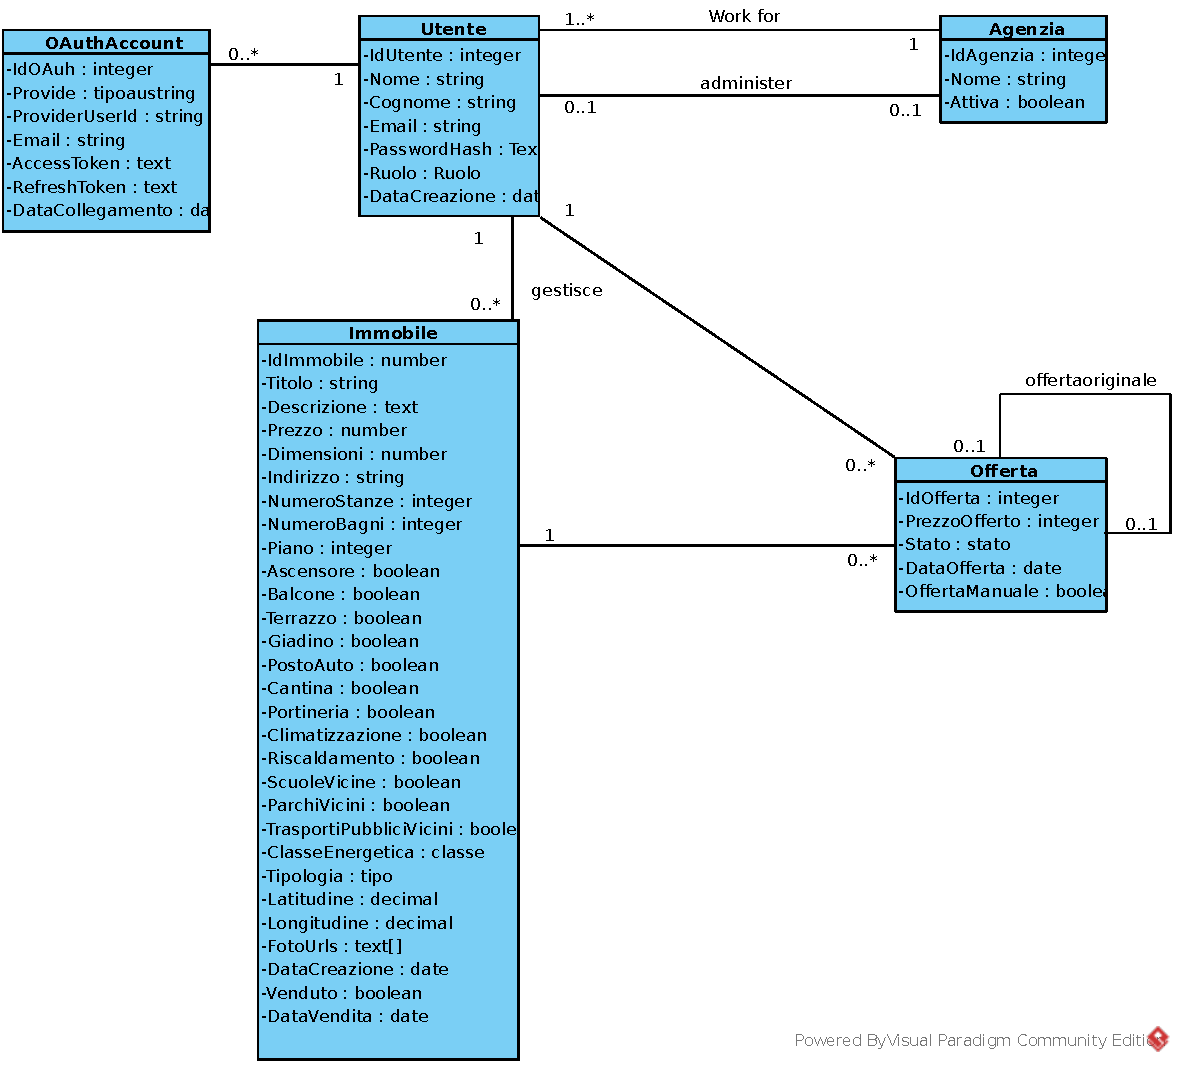
\includegraphics[width=\textwidth]{database_ristrutturatobuono.pdf}
    \caption{Database}
    \label{Database}
\end{figure}

\newpage
\subsection{Descrizione e motivazione delle scelte di design dell'interfaccia utente}

Il design dell'interfaccia utente (UI) è un pilastro del progetto, guidato dall'obiettivo di qualità: \textbf{Usabilità}. L'obiettivo è un'applicazione intuitiva, rapida e accessibile sia a clienti privati che ad amministratori.

\subsection{Analisi sugli attributi di qualità di Nielsen}
La progettazione ha bilanciato i cinque attributi di qualità di Nielsen focalizzandosi su:

\subsubsection{Learnability e Memorability}
Individuate come priorità data l'eterogeneità degli utenti. Si è scelto di utilizzare pattern di navigazione standard e scritte per rendere l'uso immediato anche per utenti sporadici.

\subsubsection{Gestione degli Errori (Errors)}
Punto focale vista la complessità del caricamento di un annuncio. Si utilizzano validazioni per prevenire l'invio di dati errati.


\subsection{Scelte Tecnologiche: Next.js e Tailwind CSS}
La scelta di \textbf{Next.js} permette un caricamento istantaneo delle pagine, migliorando la \textit{perceived performance}. L'uso di \textbf{Tailwind CSS} garantisce:
\begin{itemize}
    \item \textbf{Consistenza:} Scala cromatica e tipografica uniforme.
\end{itemize}

\subsection{Principi di Design e HCI}

\subsubsection{Affordances}
L'apparenza degli elementi suggerisce l'uso. Alcuni pulsanti di azione (Login, Cerca) sono realizzati in \textbf{colore Rosso} , simulando la "cliccabilità" fisica e guidando l'occhio verso le azioni primarie.

\subsubsection{Constraints (Vincoli)}
L’interfaccia adotta vincoli proattivi basati sul profilo utente, impedendo errori di sottomissione tramite validazione real-time e garantendo che ogni attore (Cliente, Agente, Supporto o Admin) possa interagire esclusivamente con le funzioni pertinenti al proprio livello di autorizzazione.

\subsubsection{Feedback (Riscontro)}
Ogni interazione riceve un riscontro visivo. Le classi di stato di Tailwind evidenziano i campi in \textit{focus} o con errori , mentre le notifiche \textit{toast} confermano il successo delle operazioni.

\subsubsection{Metaphors e Mappings}
Le metafore adottate non sono esclusivamente iconografiche, ma concettuali: l'uso di \textit{Cards} per gli annunci richiama le schede informative fisiche delle agenzie immobiliari, rendendo l'interfaccia familiare e riducendo lo sforzo cognitivo

\subsection{Modelli Predittivi e Cognitivi}

\subsubsection{Legge di Hick}
Per ridurre il tempo di decisione, i filtri complessi sono raggruppati in menu collassabili, evitando di sovraccaricare l'utente con troppe scelte simultanee.

\subsubsection{Legge di Fitts}
Le \textit{Call to Action} (CTA) sono di dimensioni generose e posizionate in aree facilmente raggiungibili, riducendo il tempo di acquisizione del target sia su desktop che su mobile.

\subsection{Visual Design: Colore e Tipografia}

\subsubsection{Strategia Cromatica}
\begin{itemize}
    \item \textbf{Colore Primario (Rosso):} Utilizzato per le azioni critiche e di conversione.
    \item \textbf{Sfondo (Bianco/Trasparente):} Garantisce pulizia visiva e risalto alle foto degli immobili.
    \item \textbf{Testo (Nero):} Alto contrasto per la massima leggibilità.
\end{itemize}

\subsubsection{Tipografia}

\subsection{Classi di design}
In questa parte della documentazione sono mostrate le classi di design del back end e front end.

\subsubsection{class design back-end}
\begin{figure}[htbp]
    \centering
    % Usa includegraphics per i file PDF
    % Assicurati che il file si chiami esattamente dietiestate-classidesign2.pdf su Overleaf
    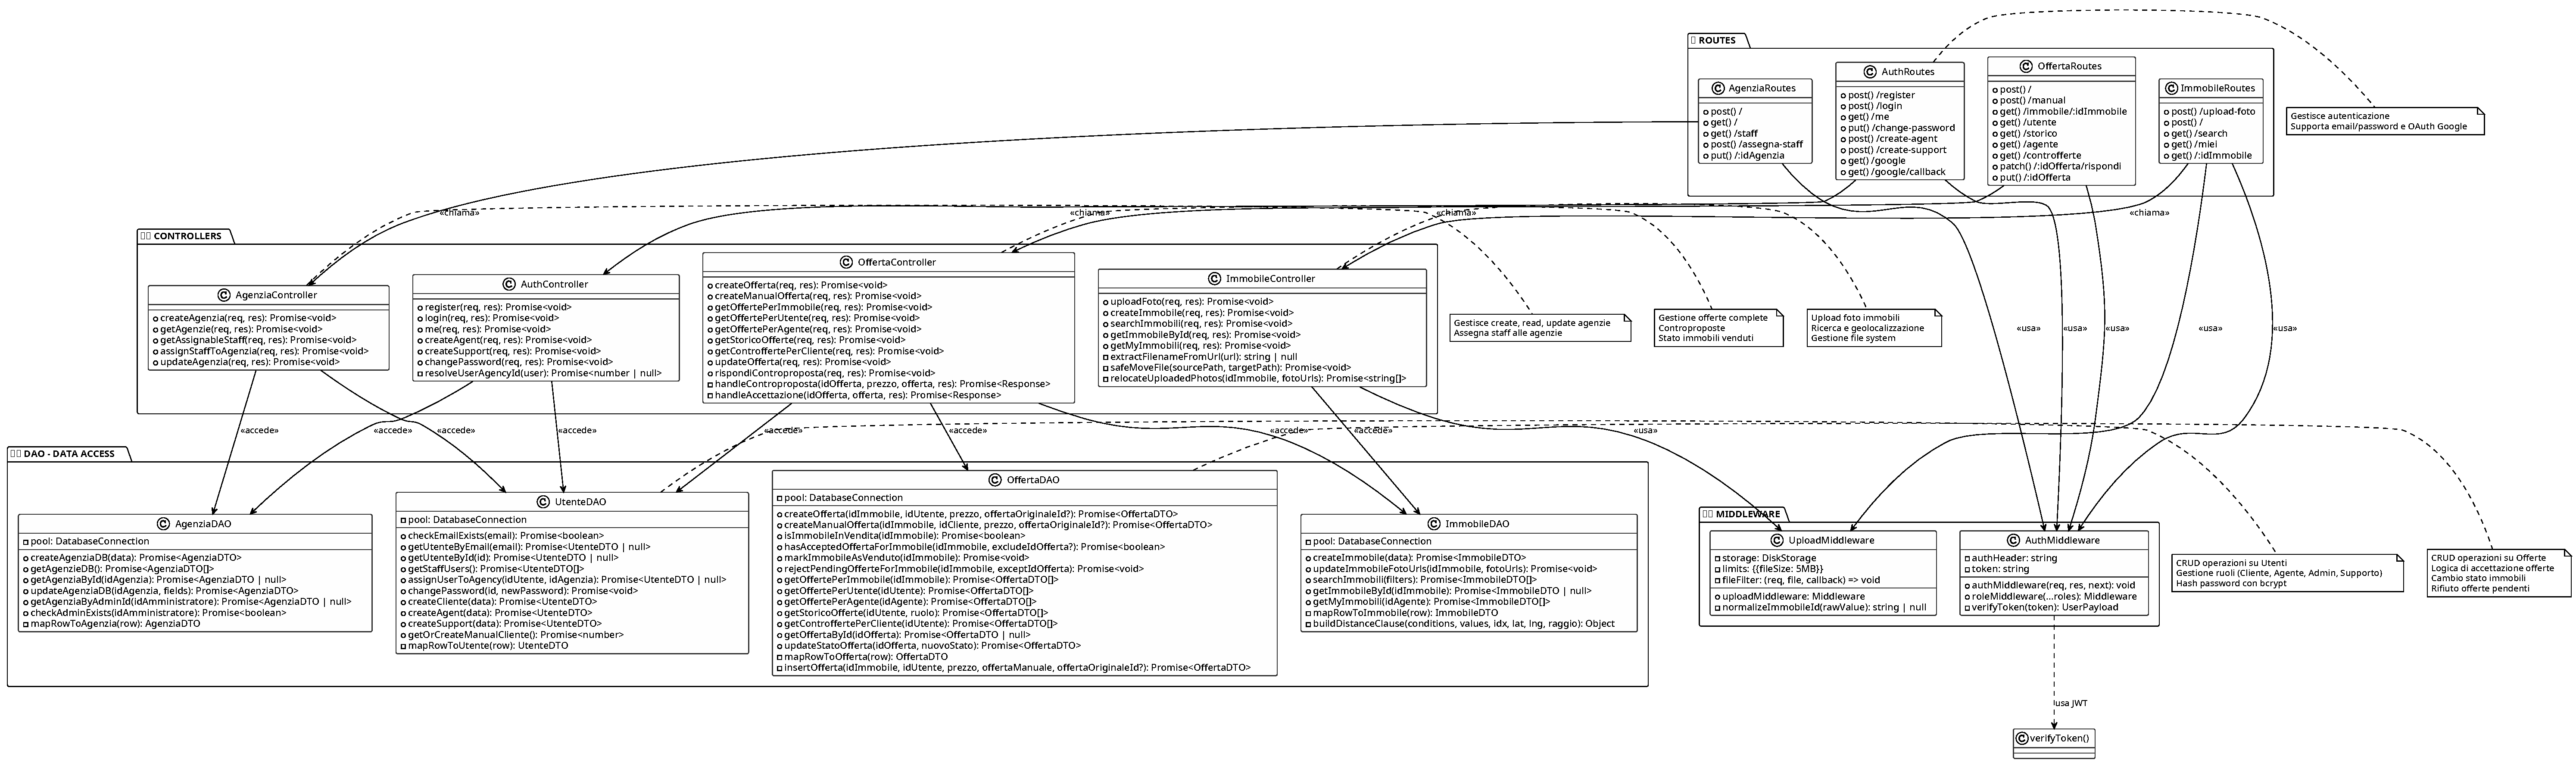
\includegraphics[width=\textwidth]{classdesign-backend.pdf}
    \caption{Back-end class design}
    \label{fig:frontend-class}
\end{figure}

\newpage
\subsubsection{class design front-end}
\begin{figure}[htbp]
    \centering
    % Usa includegraphics per i file PDF
    % Assicurati che il file si chiami esattamente dietiestate-classidesign2.pdf su Overleaf
    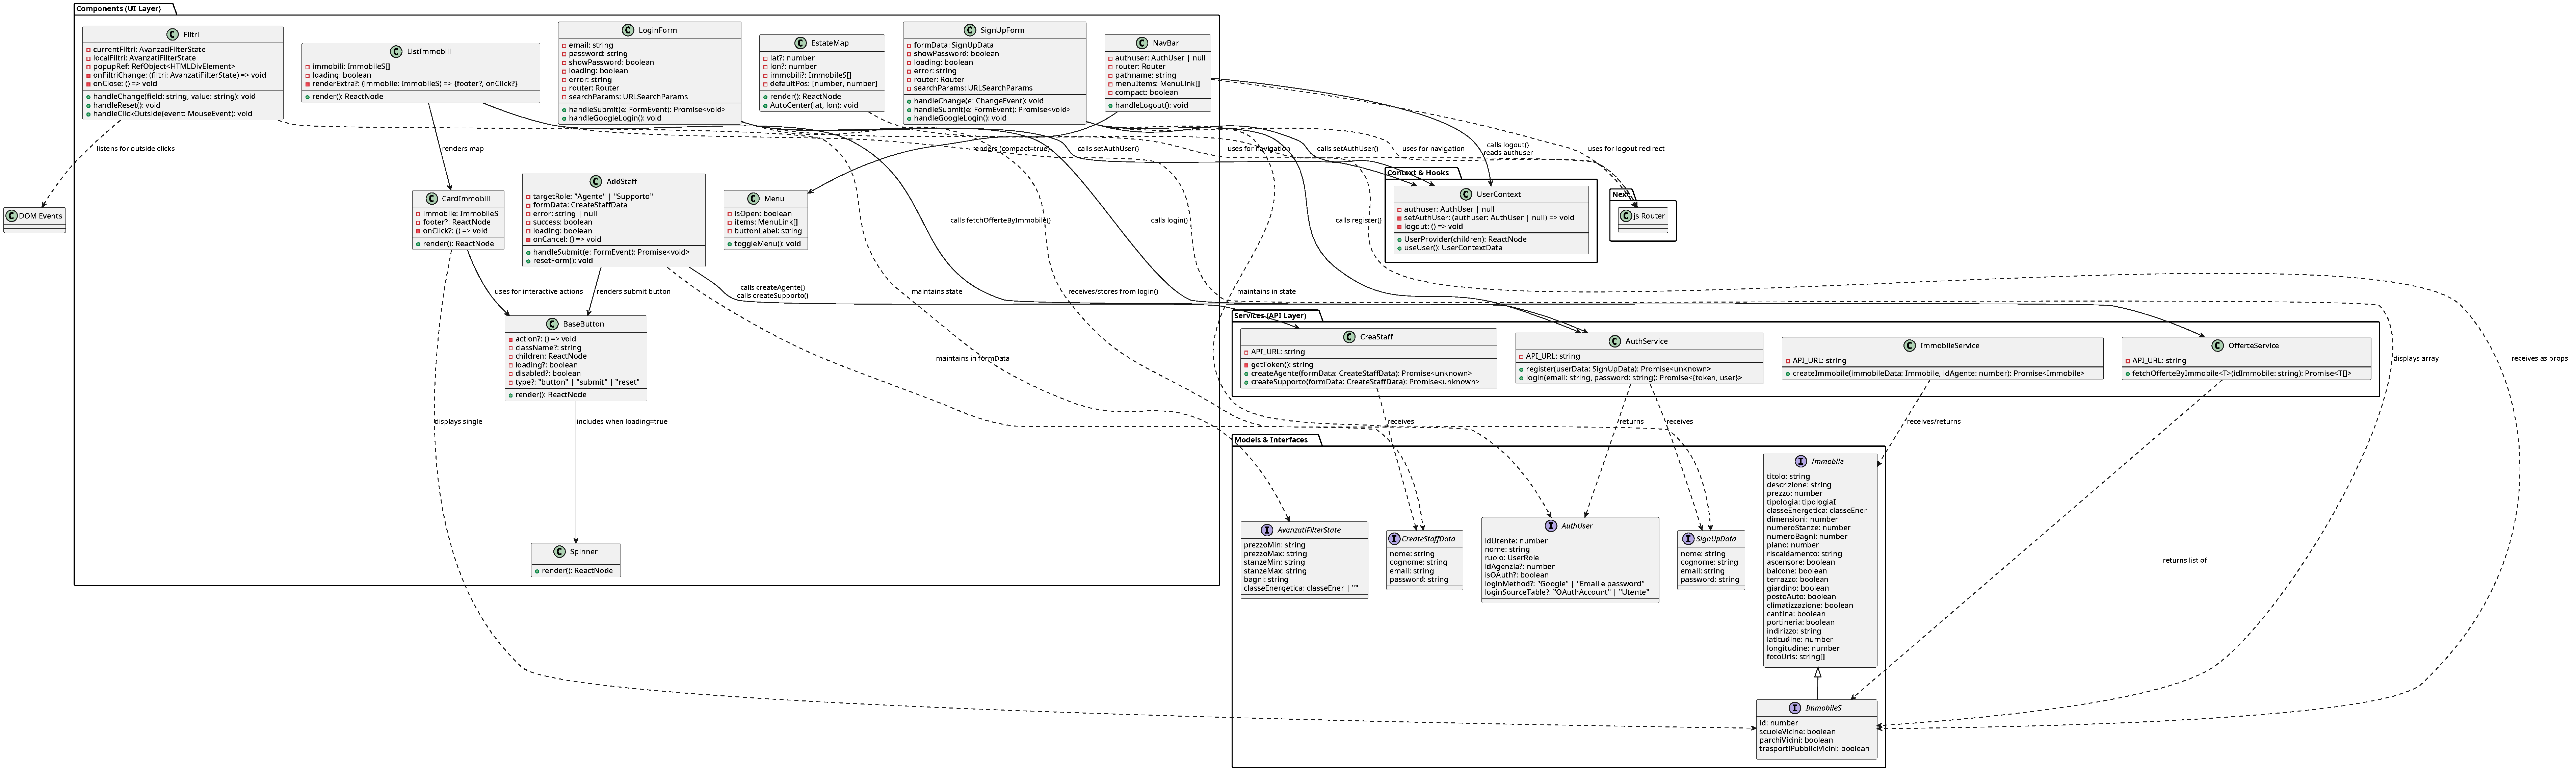
\includegraphics[width=\textwidth]{dietiestates-classdesign2.pdf}
    \caption{front-end class design}
    \label{fig:frontend-class}
\end{figure}

\newpage


\begin{figure}[htbp]
    \centering
    % Usa includegraphics per i file PDF
    % Assicurati che il file si chiami esattamente dietiestate-classidesign2.pdf su Overleaf
    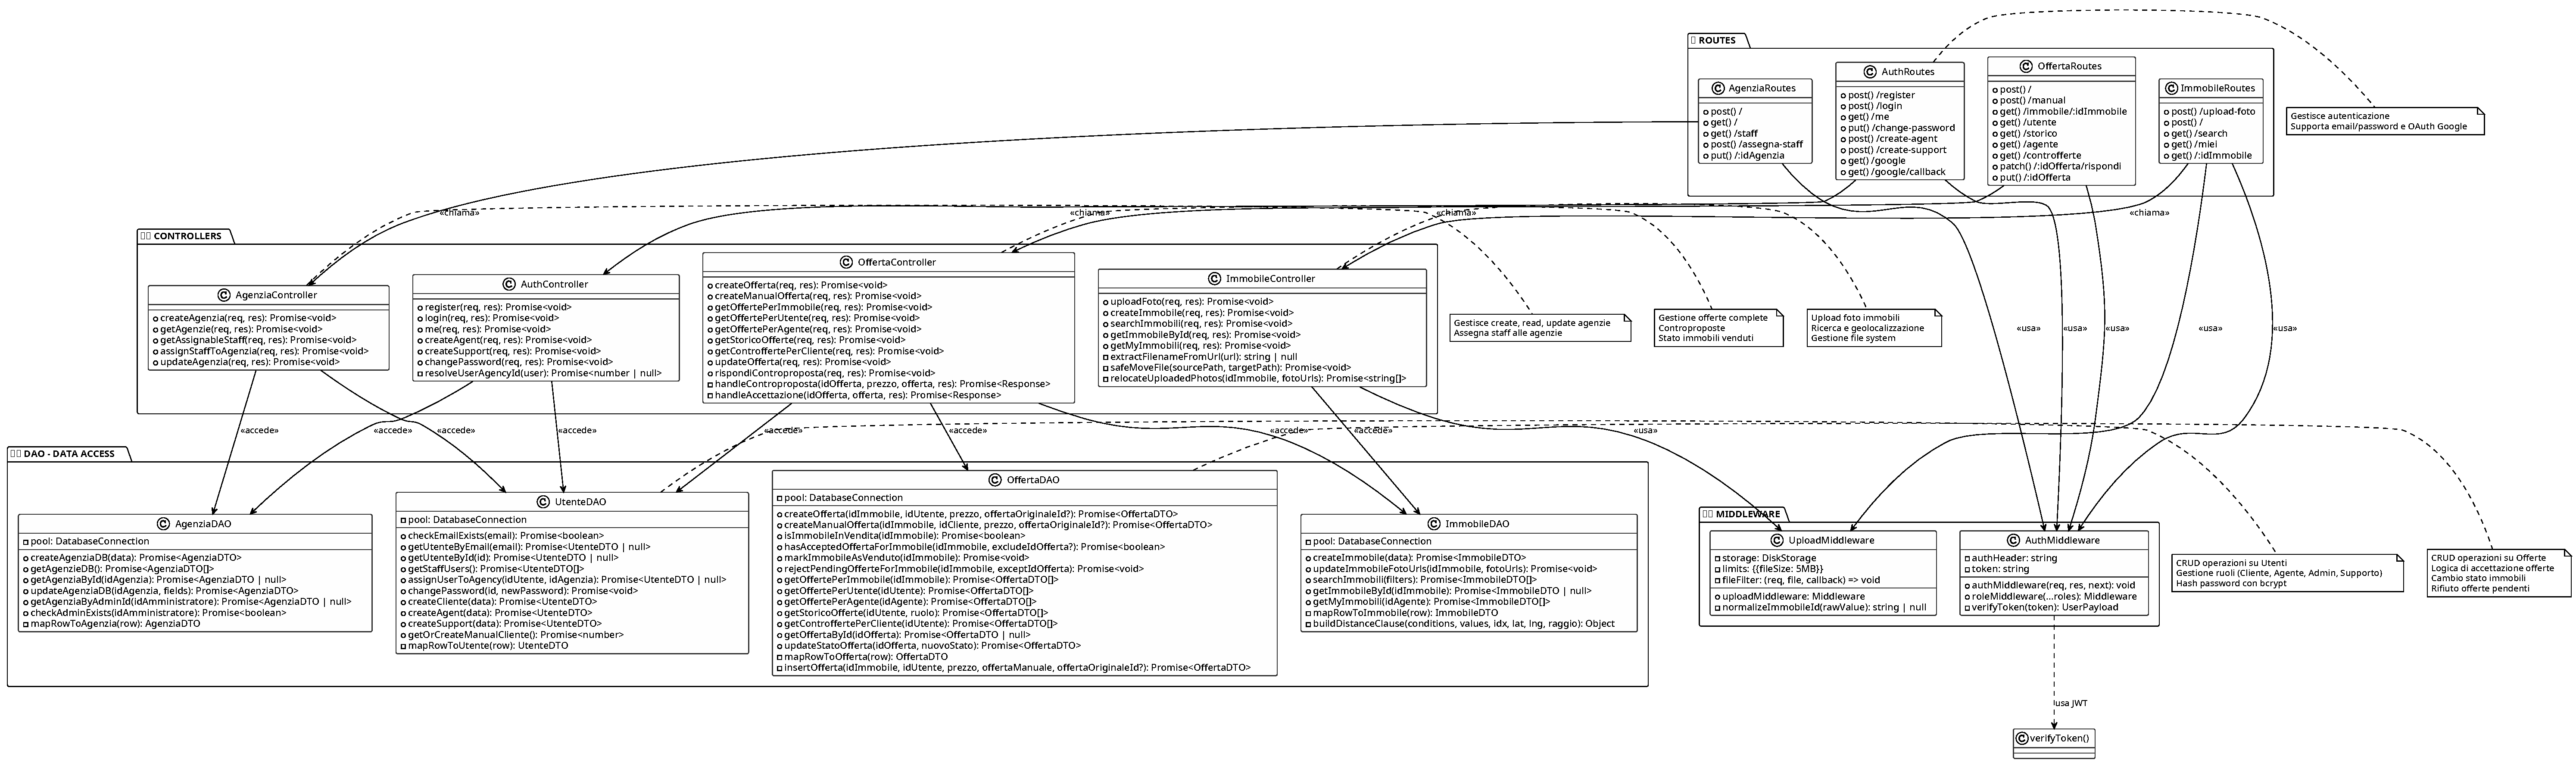
\includegraphics[width=\textwidth]{classdesign-backend.pdf}
    \caption{Back-end class design}
    \label{fig:frontend-class}
\end{figure}
\newpage
\subsection{Sequenze diagram}
In questa sezione viene illustrata la dinamica del sistema attraverso i Diagrammi di Sequenza riferiti al punto sugli use case.
\newpage
\subsubsection{Crea agente}
\begin{figure}[htbp]
    \centering
    % Usa includegraphics per i file PDF
    % Assicurati che il file si chiami esattamente dietiestate-classidesign2.pdf su Overleaf
    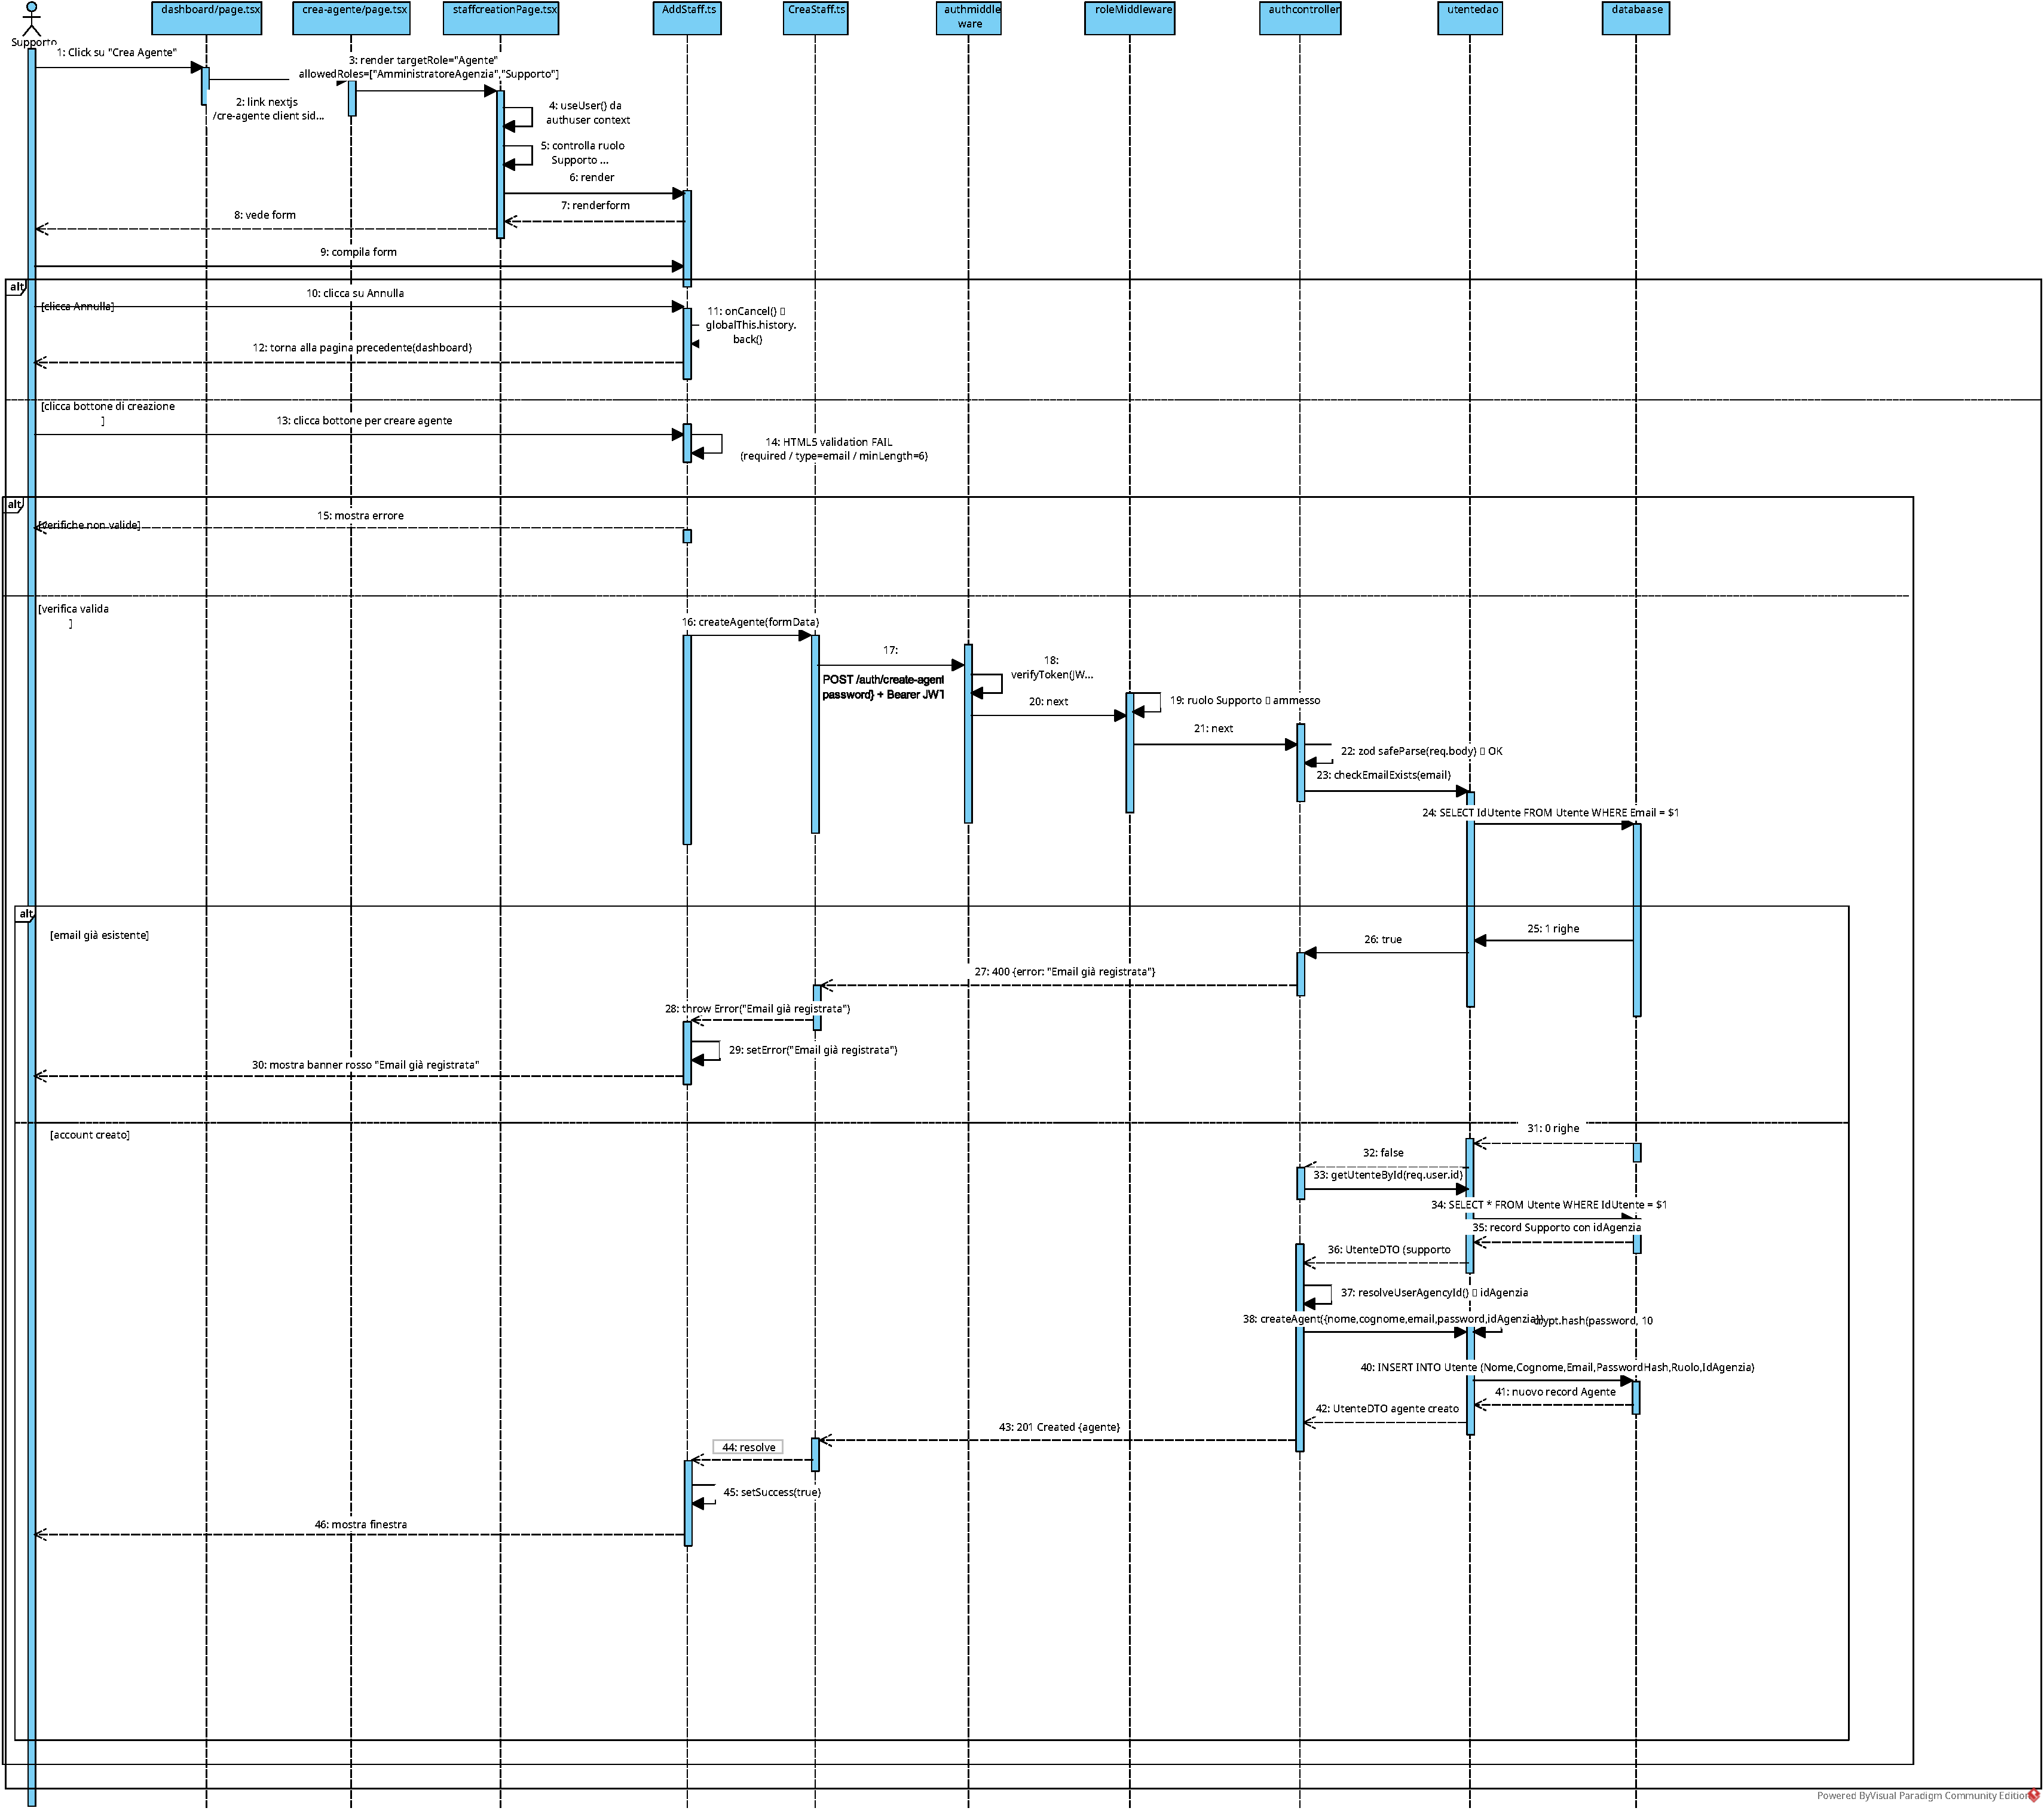
\includegraphics[width=\textwidth]{Sequence Diagram crea agente.pdf}
    \caption{crea agente}
    \label{crea agente}
\end{figure}
\newpage

\subsubsection{Crea supporto}
\begin{figure}[htbp]
    \centering
    % Usa includegraphics per i file PDF
    % Assicurati che il file si chiami esattamente dietiestate-classidesign2.pdf su Overleaf
    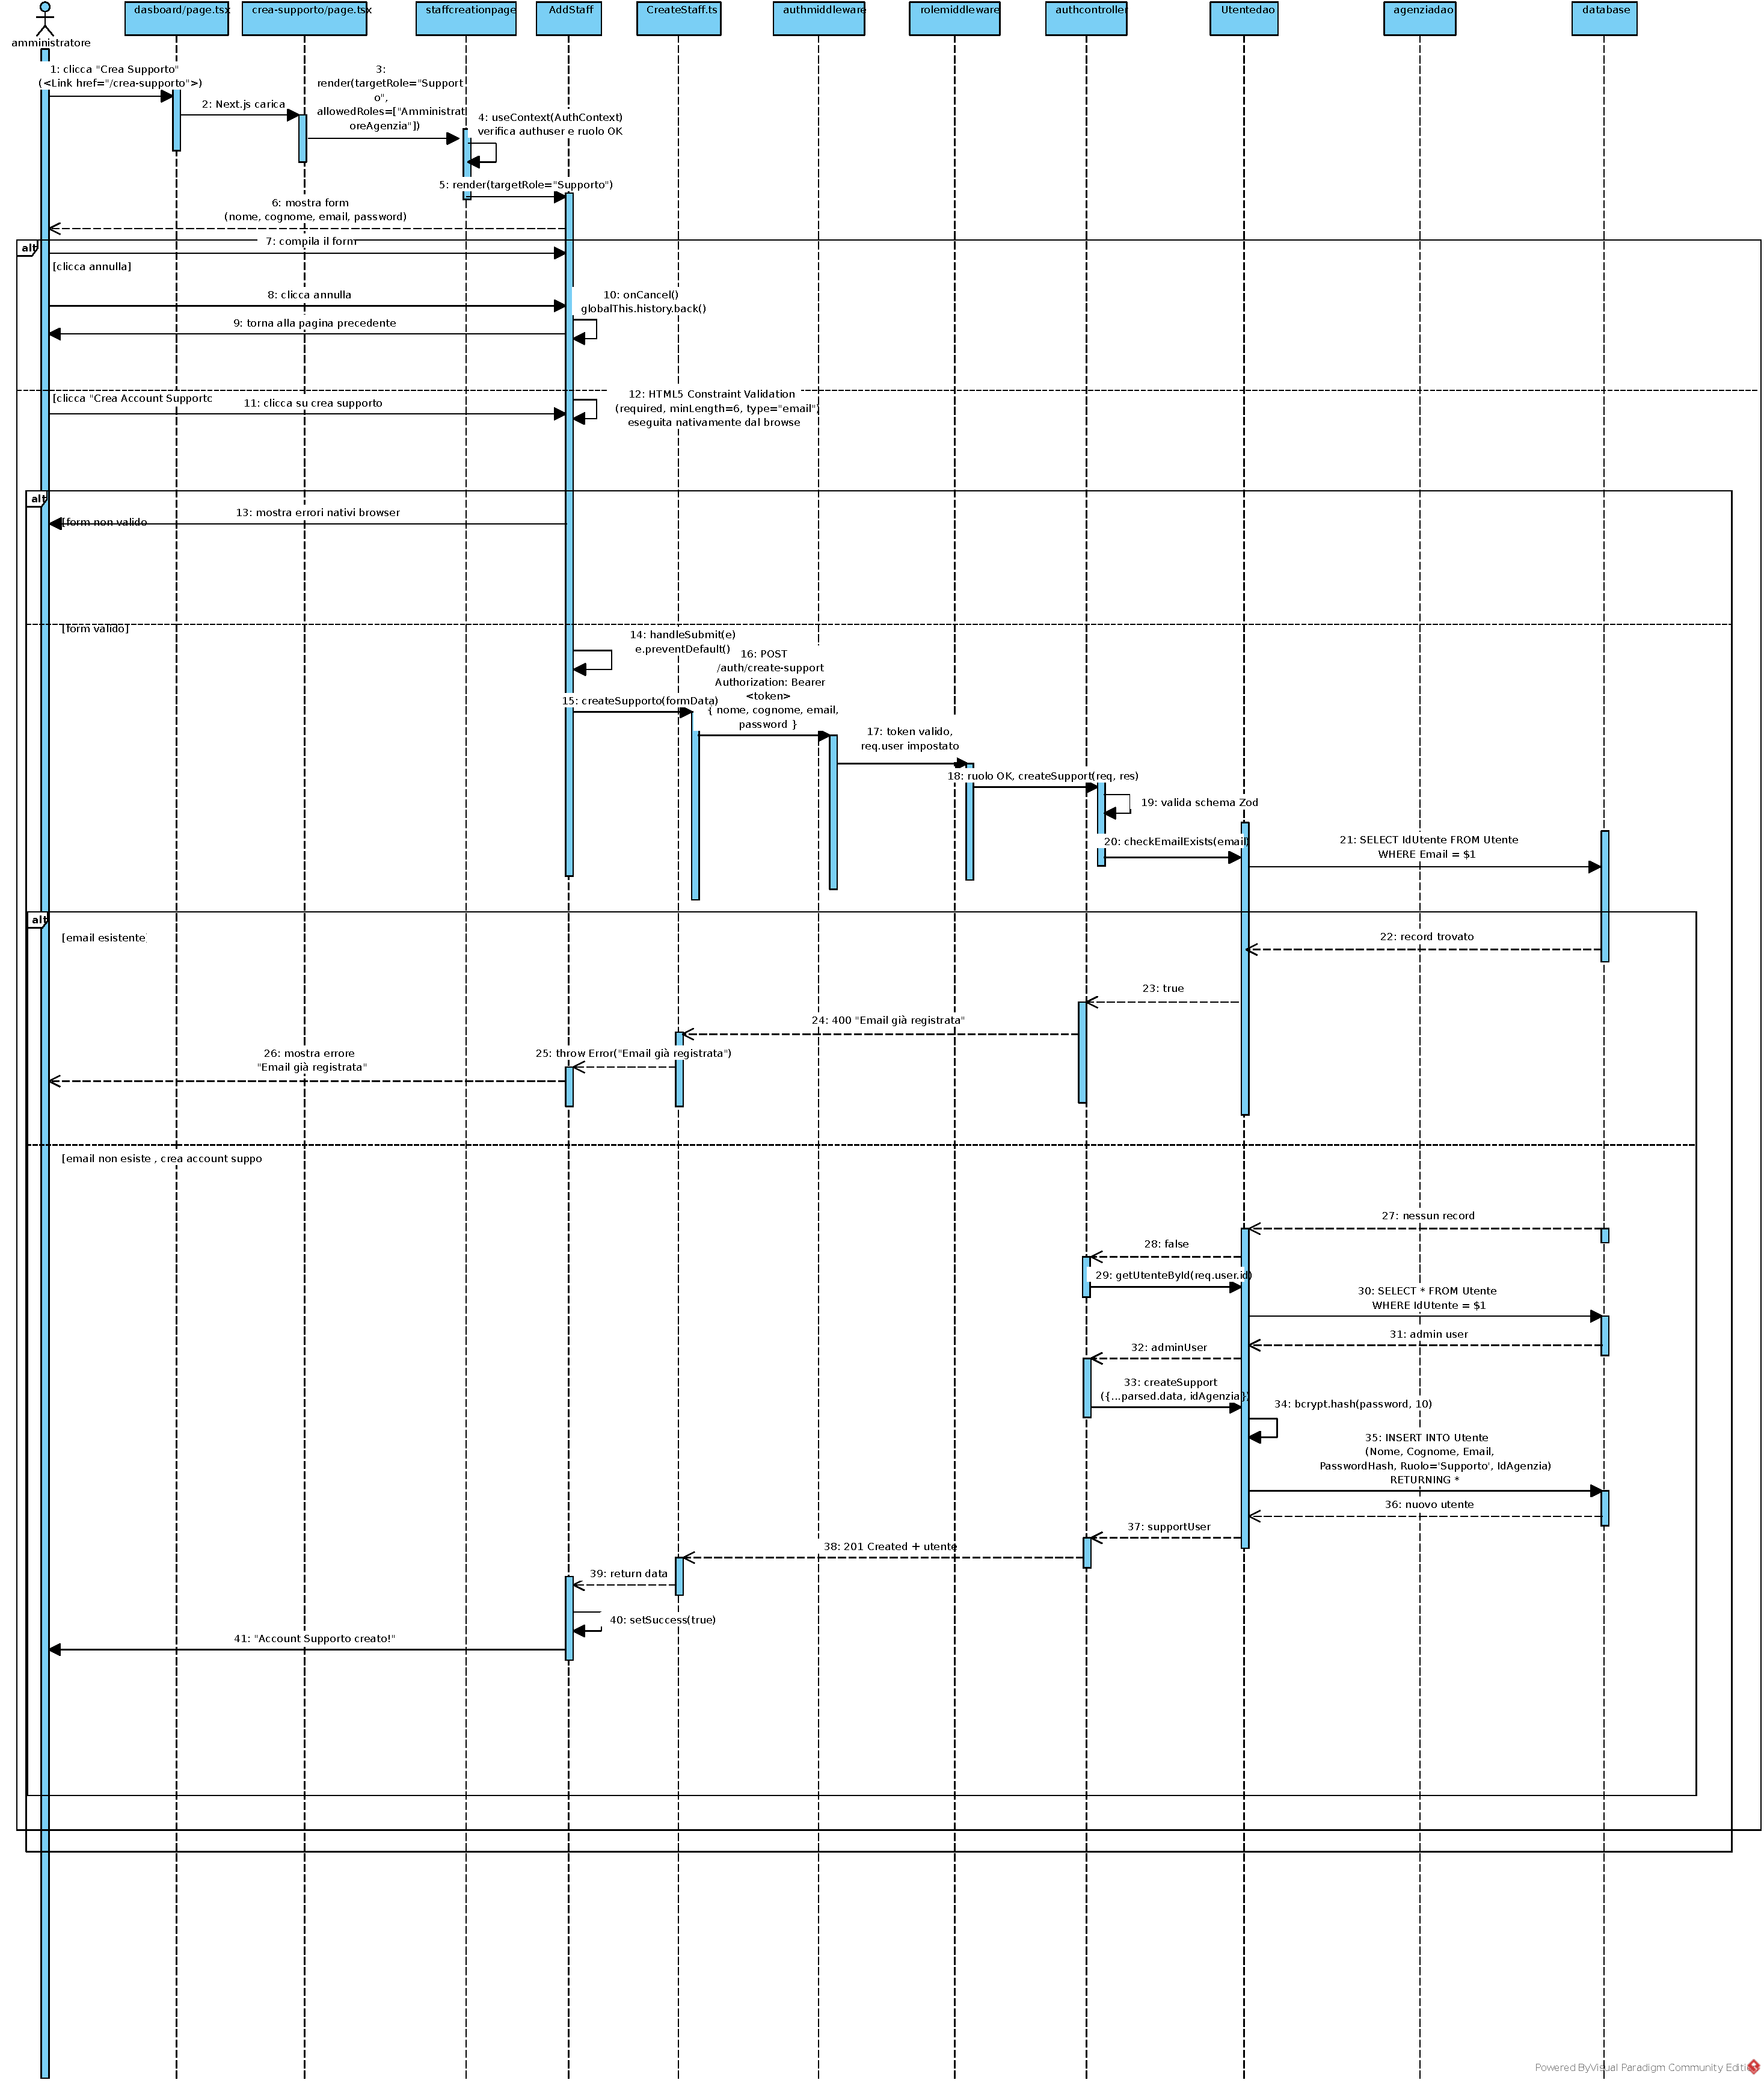
\includegraphics[width=\textwidth]{Sequence Diagram creazione supporto.pdf}
    \caption{crea supporto}
    \label{crea supporto}
\end{figure}
\newpage
\subsubsection{Offerta manuale}
\begin{figure}[htbp]
    \centering
    % Usa includegraphics per i file PDF
    % Assicurati che il file si chiami esattamente dietiestate-classidesign2.pdf su Overleaf
    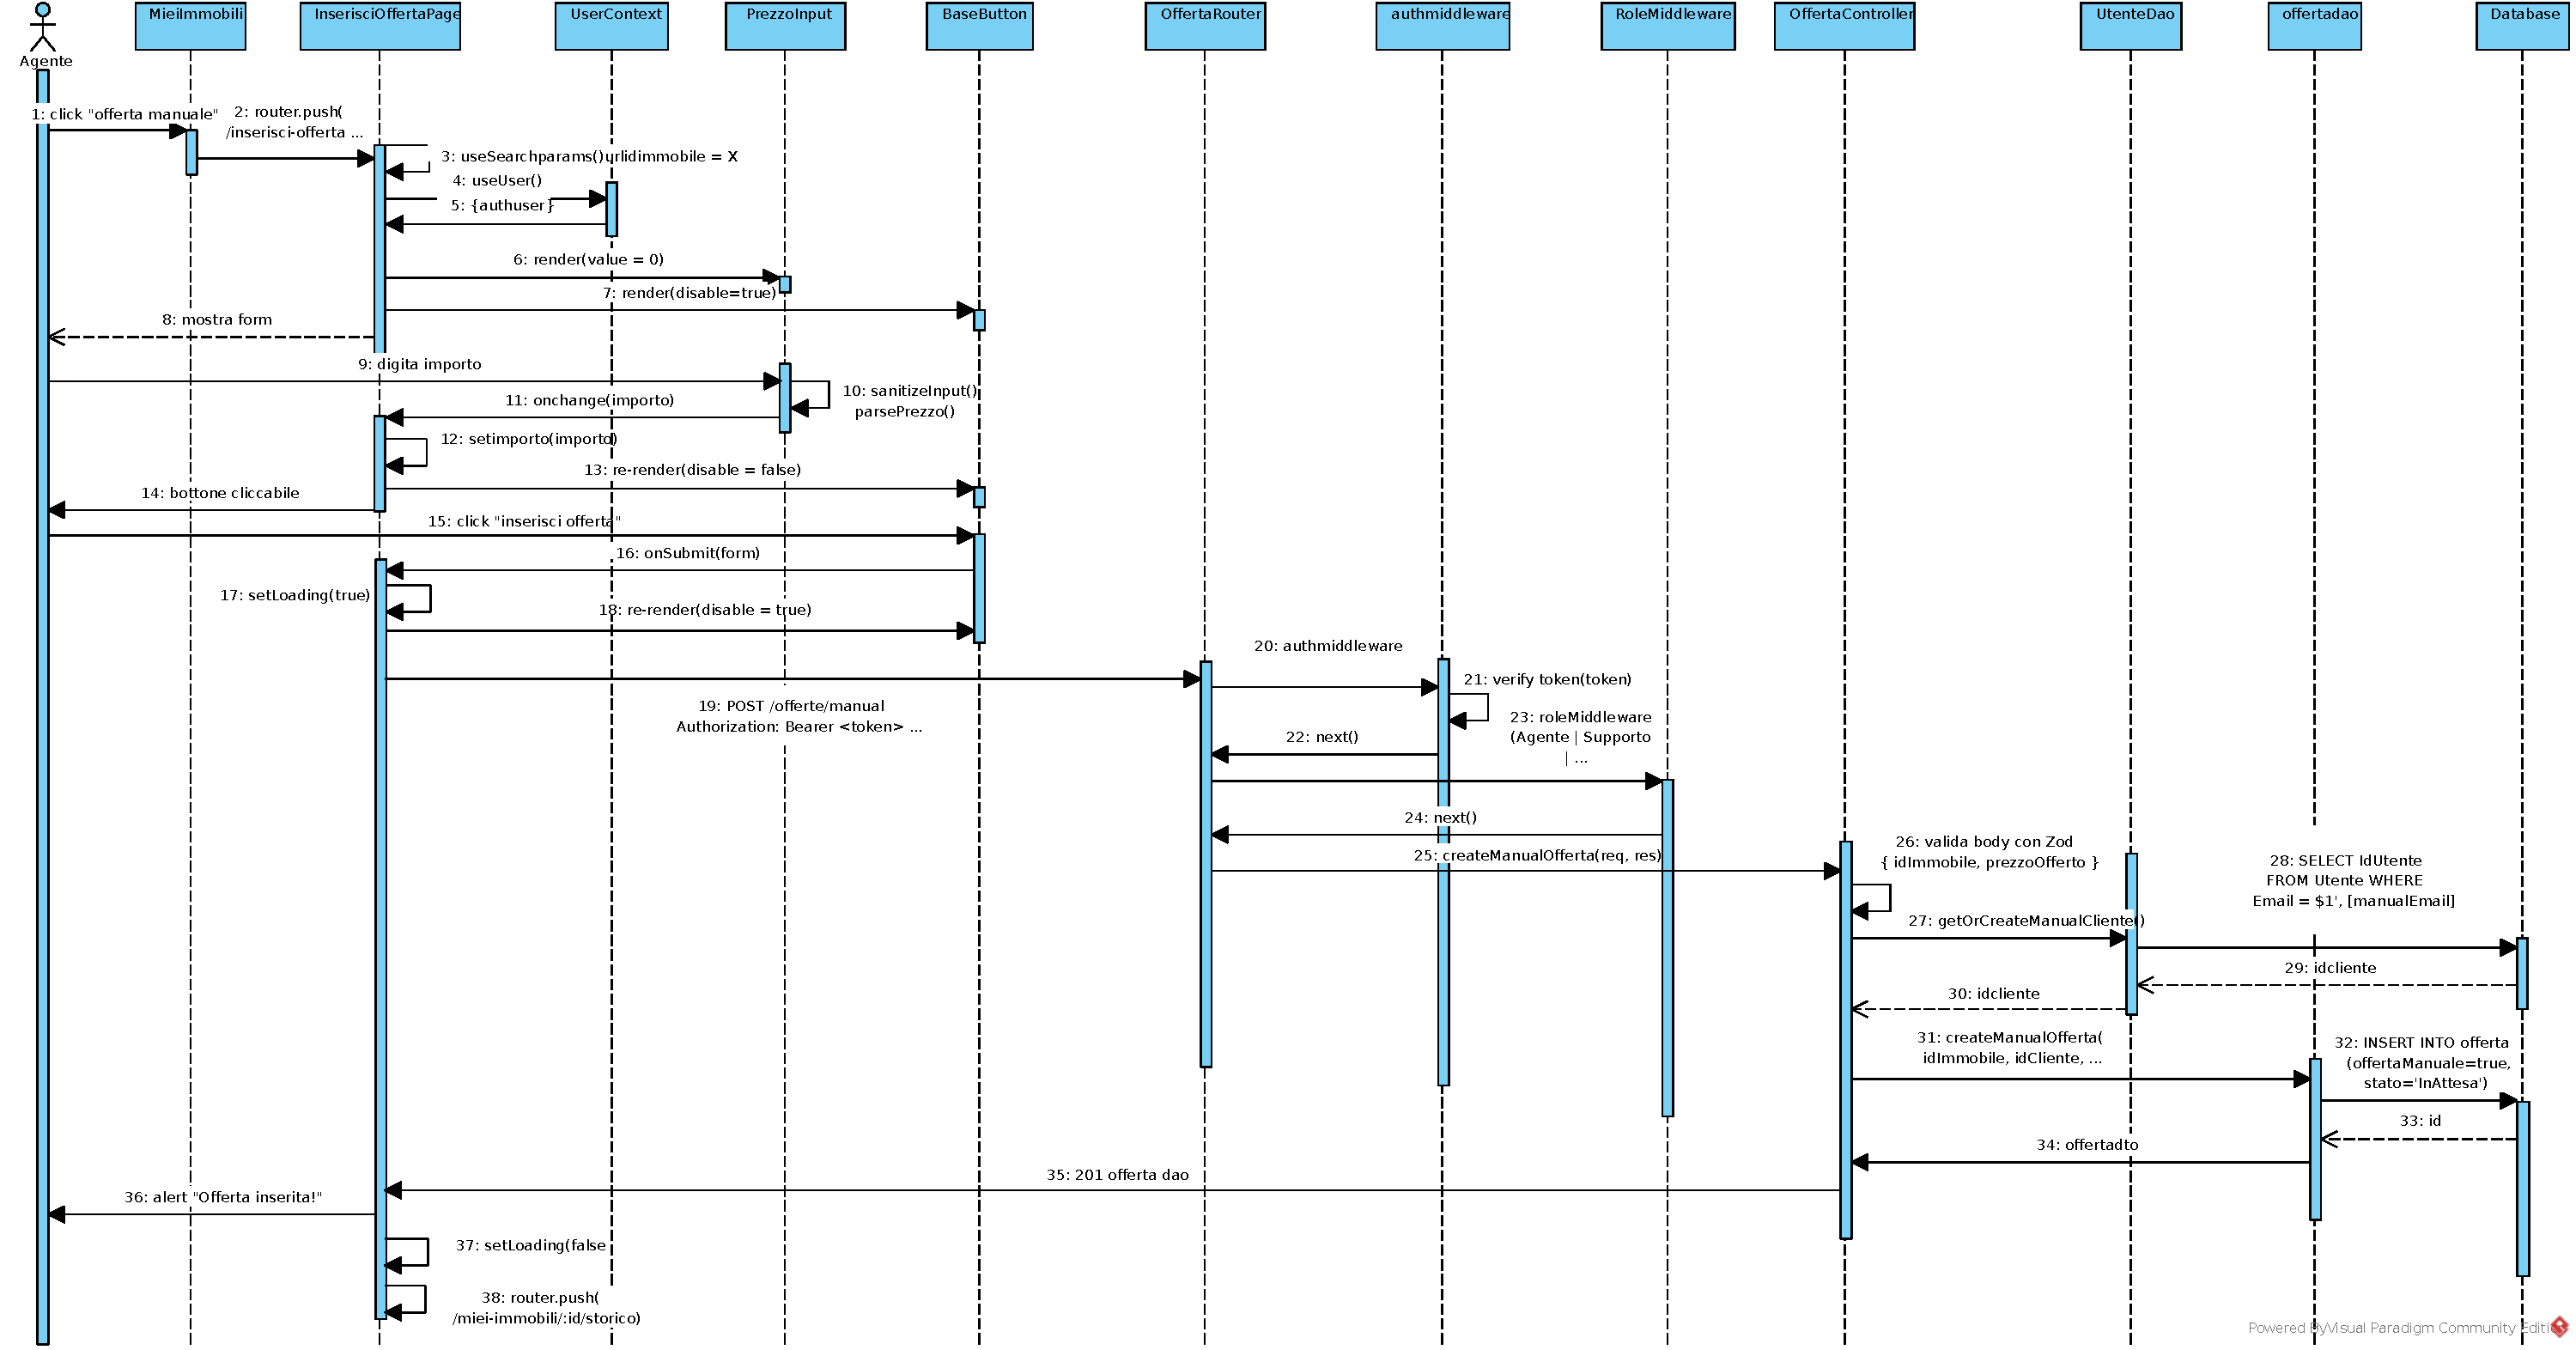
\includegraphics[width=\textwidth]{Sequence Diagram Offerta manuale.pdf}
    \caption{Offerta manuale}
    \label{Offerta manuale}
\end{figure}
\newpage

\subsubsection{visualizza immobile}
\begin{figure}[htbp]
    \centering
    % Usa includegraphics per i file PDF
    % Assicurati che il file si chiami esattamente dietiestate-classidesign2.pdf su Overleaf
    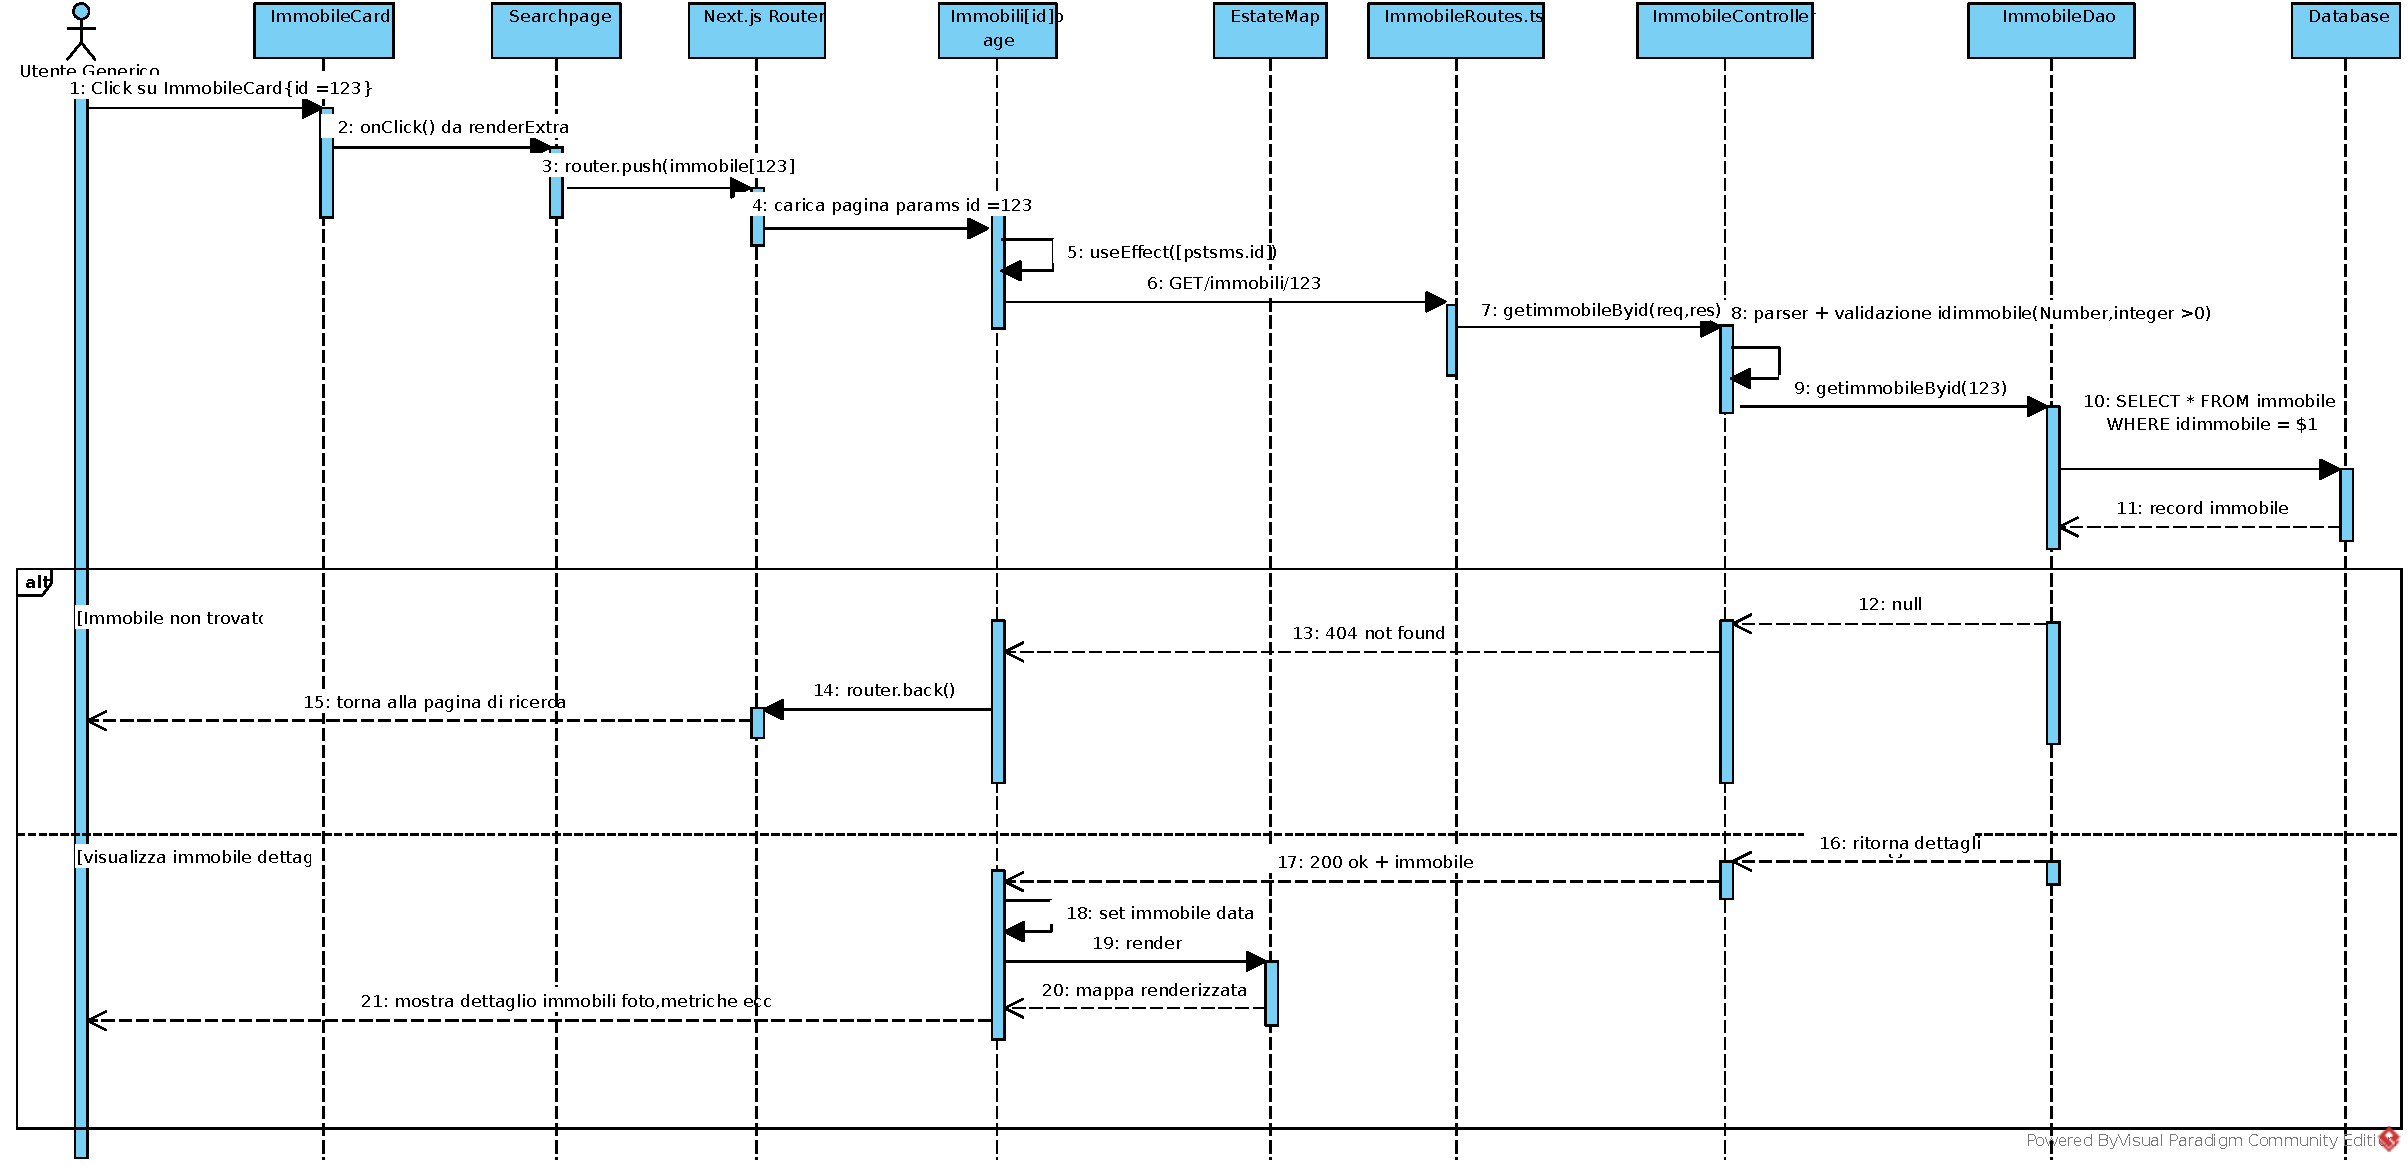
\includegraphics[width=\textwidth]{Sequence Diagram Dietiestates.pdf}
    \caption{visualizza immobile}
    \label{visualizza immobile}
\end{figure}
\newpage
\section{Artefatti Software e documentazione del processo di sviluppo}
Al fine di garantire elevati standard di affidabilità, manutenibilità e sicurezza del software sviluppato, il progetto è stato sottoposto a cicli sistematici di Analisi Statica del Codice (Static Application Security Testing - SAST). Per tale scopo è stato integrato nella pipeline di sviluppo SonarQube, una piattaforma leader nel settore per l'ispezione continua della qualità del codice. Nelle sezioni seguenti verranno analizzati i report generati, con particolare attenzione alle metriche di Reliability, Security e Maintainability.

\begin{figure}[htbp]
    \centering
    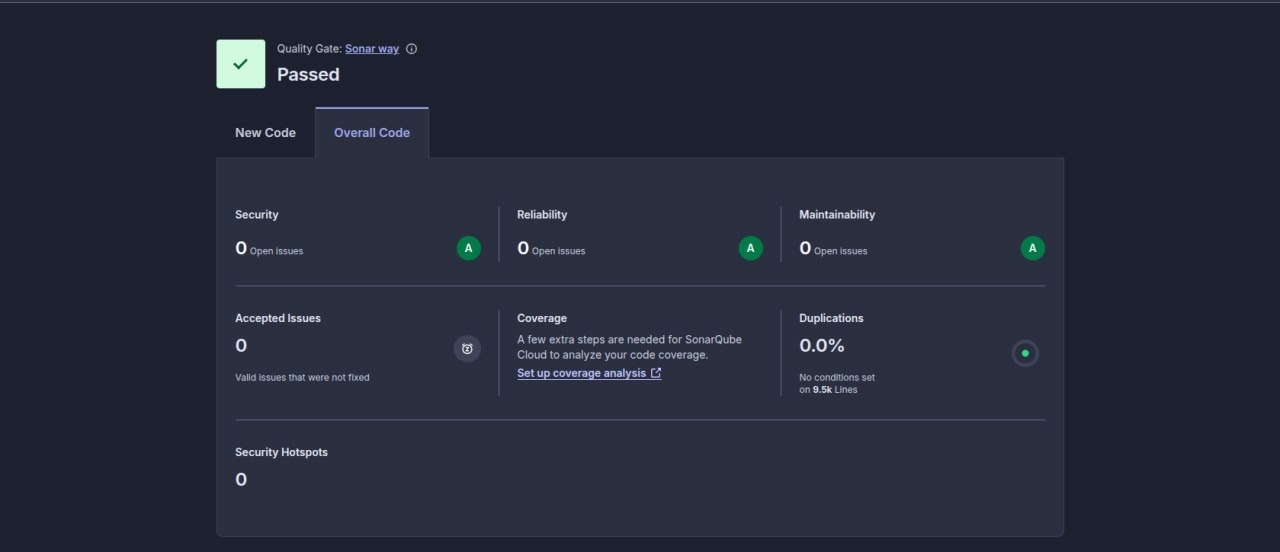
\includegraphics[width=0.8\textwidth]{sonarqube.jpg}
    \caption{Report della qualità del codice generato da SonarQube.}
    \label{fig:sonarqube_report}
\end{figure}

\newpage
\subsection{Report di qualità del codice, generati da SonarQube}
\section{Testing e valutazione dell’usabilità.}

\subsection{Expert Review}
La valutazione è stata condotta tramite ispezione euristica, usando le \textbf{10 euristiche di Nielsen} come base della checklist, adattate alle funzionalità specifiche di DietiEstates25.

\subsubsection{Checklist di Usabilità}

\begin{enumerate}
    \item \textbf{Visibilità dello Stato del Sistema}
    \begin{itemize}
        \item L'utente riceve un feedback immediato per ogni azione eseguita (es. indicatori di caricamento, messaggi di conferma)?
        \item Lo stato di avanzamento nei processi complessi è sempre chiaramente indicato (es. stepper per form multi-fase)?
        \item Il sistema comunica visivamente eventuali ritardi causati da servizi esterni o caricamento dati?
    \end{itemize}

    \item \textbf{Corrispondenza col Mondo Reale}
    \begin{itemize}
        \item La terminologia utilizzata è familiare all'utente e coerente con il dominio applicativo?
        \item Le icone e le metafore visive sono intuitive e universalmente riconoscibili nel contesto d'uso?
    \end{itemize}

    \item \textbf{Controllo e Libertà dell'Utente}
    \begin{itemize}
        \item L'utente può annullare, correggere o resettare le proprie azioni senza perdita di dati non necessaria?
        \item È possibile navigare liberamente tra le diverse fasi di un processo lineare (es. tasti "Avanti" e "Indietro")?
        \item Esistono vie d'uscita chiaramente contrassegnate per abbandonare uno stato indesiderato?
    \end{itemize}

    \item \textbf{Consistenza e Standard}
    \begin{itemize}
        \item Il linguaggio e la terminologia sono coerenti in tutte le sezioni dell'interfaccia?
        \item Il layout, i colori e i componenti grafici seguono standard visivi uniformi per tutti i ruoli utente?
    \end{itemize}

    \item \textbf{Prevenzione degli Errori}
    \begin{itemize}
        \item Il sistema impedisce attivamente azioni errate (es. disabilitando pulsanti se i vincoli non sono rispettati)?
        \item I vincoli e i campi obbligatori sono comunicati chiaramente prima che l'utente commetta un errore?
    \end{itemize}

    \item \textbf{Riconoscimento piuttosto che Richiamo}
    \begin{itemize}
        \item Le informazioni necessarie (es. filtri attivi o dati inseriti precedentemente) sono sempre visibili o facilmente reperibili?
        \item L'interfaccia riduce il carico mnemonico dell'utente proponendo opzioni di scelta visibili (es. menu a tendina, checkbox)?
    \end{itemize}

    \item \textbf{Flessibilità ed Efficienza}
    \begin{itemize}
        \item L'interfaccia è ottimizzata per i diversi profili utente, offrendo funzionalità specifiche per ogni ruolo?
        \item Sono presenti "acceleratori" (es. azioni rapide, scorciatoie) per velocizzare le operazioni più frequenti?
        \item Il sistema offre diverse modalità di interazione per soddisfare sia l'utente inesperto che quello avanzato?
    \end{itemize}

    \item \textbf{Design Minimalista}
    \begin{itemize}
        \item Le schermate mostrano solo le informazioni essenziali per il compito corrente, evitando il sovraccarico visivo?
        \item L'interfaccia è priva di elementi decorativi o informativi ridondanti che potrebbero distrarre l'utente?
    \end{itemize}

    \item \textbf{Gestione e Recupero degli Errori}
    \begin{itemize}
        \item I messaggi di errore sono espressi in linguaggio semplice, indicano con precisione il problema e suggeriscono una soluzione?
        \item In caso di guasto dei servizi di terze parti, il sistema fornisce un feedback comprensibile invece di bloccarsi?
        \item Gli errori sono segnalati in prossimità del punto in cui si sono verificati per facilitarne la correzione?
    \end{itemize}

    \item \textbf{Guida e Documentazione}
    \begin{itemize}
        \item Il sistema fornisce aiuti contestuali e indicazioni chiare sulla compilazione dei dati (es. tooltip, placeholder)?
        \item La navigazione permette all'utente di orientarsi facilmente, indicando chiaramente la posizione attuale all'interno dell'applicazione?
    \end{itemize}
\end{enumerate}
\newpage
\subsubsection{Applicazione della checklist al prodotto}

\subsubsection*{Autenticazione (Login e Registrazione)}

\textbf{Punti di forza:}
\begin{itemize}
    \item Il messaggio di errore appare comunque, quindi l'utente sa che qualcosa è andato storto.
    \item \textbf{Controllo e libertà dell'utente:} È presente il pulsante ``mostra password'', che permette all'utente di verificare quanto sta digitando prima di confermare.
\end{itemize}

\textbf{Criticità:}
\begin{itemize}
    \item \textbf{Gestione errori:} Il messaggio di errore è generico (es. ``autenticazione fallita'') e non specifica la causa del problema.
    \item \textbf{Prevenzione degli errori:} I campi obbligatori non sono chiaramente indicati, manca un segnale visivo come l'asterisco (*).
    \item \textbf{Guida e documentazione:} Nessun requisito sulla password viene comunicato all'utente (es. lunghezza minima, caratteri richiesti).
\end{itemize}

\subsubsection*{Navbar}

\textbf{Punti di forza:}
\begin{itemize}
    \item \textbf{Flessibilità ed efficienza:} La navbar si adatta al ruolo dell'utente autenticato, mostrando solo le voci pertinenti (cliente, agente, admin, supporto).
    \item \textbf{Corrispondenza col mondo reale:} Le voci di navigazione sono chiare e visibili, senza ambiguità terminologiche.
\end{itemize}

\textbf{Criticità:}
\begin{itemize}
    \item \textbf{Visibilità dello stato:} La navbar non indica chiaramente in quale sezione si trova l'utente. Non è presente un segnale visivo (es. voce evidenziata, sottolineatura o colore diverso) sulla pagina corrente, rendendo difficile l'orientamento durante la navigazione.
\end{itemize}
\subsubsection*{Inserimento Immobile}

\textbf{Punti di forza:}
\begin{itemize}
    \item \textbf{Design minimalista:} Il form è diviso in step logici, presentando un sottoinsieme di informazioni alla volta e riducendo il carico cognitivo dell'utente.
    \item \textbf{Controllo e libertà dell'utente:} L'utente può navigare liberamente avanti e indietro tra gli step senza perdere i dati già inseriti.
\end{itemize}

\textbf{Criticità:}
\begin{itemize}
    \item \textbf{Prevenzione degli errori:} Il sistema non indica i campi obbligatori mancanti prima di consentire il passaggio allo step successivo. L'utente scopre le omissioni solo al momento della pubblicazione, ed è costretto a navigare tra gli step per individuare i campi mancanti senza alcuna indicazione su dove si trovino.
\end{itemize}

\subsubsection*{Ricerca (Filtri e Mappa)}

\textbf{Punti di forza:}
\begin{itemize}
    \item \textbf{Design minimalista:} La pagina di ricerca è semplice e pulita, rendendo la funzione principale immediatamente accessibile anche per utenti con poca esperienza.
\end{itemize}

\textbf{Criticità:}
\begin{itemize}
    \item \textbf{Riconoscimento piuttosto che richiamo:} Dopo aver applicato i filtri il pannello si chiude, e non è presente un riepilogo visivo dei filtri attivi. L'utente è costretto a riaprire il pannello per ricordare cosa ha impostato.
    \item \textbf{Gestione e recupero degli errori:} I suggerimenti restituiti dal servizio di geocodifica possono apparire duplicati nel dropdown, senza che il sistema li filtri o segnali il problema all'utente, generando confusione nella scelta.
\end{itemize}

\subsubsection{Progettazione e conduzione di un esperimento con utenti reali o potenziali per la
valutazione dell'usabilità del sistema realizzato}

\paragraph{Descrizione dei soggetti reclutati}
Sono stati reclutati 5 partecipanti, selezionati per rappresentare un campione 
eterogeneo in termini di età, familiarità con la tecnologia ed esperienza con 
applicazioni immobiliari.

\begin{table}[H]
\centering
\renewcommand{\arraystretch}{1.5}
\begin{tabular}{|c|l|l|c|l|l|}
\hline
\rowcolor[HTML]{010066}
{\color{white}\textbf{ID}} & {\color{white}\textbf{Nome}} & {\color{white}\textbf{Profilo}} & {\color{white}\textbf{Età}} & {\color{white}\textbf{Exp. digitale}} & {\color{white}\textbf{Exp. app imm.}} \\
\hline
U1 & Luca M.     & Studente universitario & 22 & Alta  & Bassa \\ \hline
U2 & Serena R.   & Impiegata              & 35 & Media & Media \\ \hline
U3 & Giuseppe T. & Agente immobiliare     & 48 & Media & Alta  \\ \hline
U4 & Rosa D.     & Pensionata             & 67 & Bassa & Bassa \\ \hline
U5 & Marco P.    & Lib. professionista    & 31 & Alta  & Media \\ \hline
\end{tabular}
\caption{Soggetti reclutati per l'esperimento}
\end{table}

\paragraph{Procedura Sperimentale}
I test sono stati condotti in un ambiente semi-controllato, con il partecipante 
davanti a un laptop con il browser già aperto sulla homepage di DietiEstates25. 
Per i task che richiedevano l'autenticazione, ai partecipanti sono state fornite 
credenziali preimpostate. È stato adottato il protocollo \textit{think-aloud}: 
i partecipanti sono stati invitati a verbalizzare pensieri e dubbi durante 
l'esecuzione. Un moderatore ha osservato senza intervenire, salvo in caso 
di blocco totale. La durata prevista era di 25--35 minuti per partecipante.

\paragraph{Task Assegnati}

\subparagraph{Task 1 -- Ricerca Immobile (Tempo target: 4 minuti)}

\textbf{Scenario:} \textit{``Stai cercando un immobile. Usa il sistema di 
ricerca per trovare annunci in una zona specifica, seleziona la tipologia 
di contratto e applica i filtri avanzati.''}

\textbf{Azioni attese:}
\begin{enumerate}
    \item Accedere alla pagina di ricerca.
    \item Inserire la posizione desiderata nel campo apposito.
    \item Selezionare la tipologia di contratto (vendita o affitto).
    \item Aprire e applicare i filtri avanzati.
    \item Avviare la ricerca.
\end{enumerate}

\textbf{Obiettivo:} Verificare la chiarezza e la fluidità del flusso di 
ricerca, e valutare se i filtri avanzati sono facilmente individuabili 
e comprensibili.

\subparagraph{Task 2 -- Inserimento Annuncio (Tempo target: 8 minuti)}

\textbf{Scenario:} \textit{``Accedi come agente e pubblica un nuovo annuncio 
immobiliare compilando tutte le informazioni richieste.''}

\textbf{Azioni attese:}
\begin{enumerate}
    \item Navigare alla pagina di inserimento immobile.
    \item Compilare il primo step con le informazioni base.
    \item Completare il secondo step con le caratteristiche dell'immobile.
    \item Completare il terzo step e pubblicare l'annuncio.
\end{enumerate}

\textbf{Obiettivo:} Valutare la fluidità del form multi-step e verificare 
se la suddivisione in passi è chiara. Osservare se la mancanza di 
validazione per step causa difficoltà o blocchi.

\subparagraph{Task 3 -- Inserimento Offerta (Tempo target: 3 minuti)}

\textbf{Scenario:} \textit{``Hai trovato un immobile di tuo interesse. 
Visualizza la scheda dell'annuncio e invia un'offerta.''}

\textbf{Azioni attese:}
\begin{enumerate}
    \item Selezionare un immobile dai risultati di ricerca.
    \item Visualizzare la scheda dettagliata dell'immobile.
    \item Compilare e inviare un'offerta.
\end{enumerate}

\textbf{Obiettivo:} Verificare se il percorso verso il form dell'offerta 
è intuitivo e se le informazioni di riferimento (es. prezzo richiesto) 
sono sufficientemente visibili durante la compilazione.

\paragraph{Questionario}

Per ciascuna domanda indica il tuo grado di accordo su una scala da 1 a 5,
dove 1 indica \textit{Per niente soddisfatto} e 5 indica \textit{Molto soddisfatto}.

\begin{enumerate}
    \item Quanto hai trovato il sistema facile da usare in generale?
    
    \textit{1 \quad 2 \quad 3 \quad 4 \quad 5}

    \item Quanto è stato semplice orientarti tra le diverse sezioni del sito?
    
    \textit{1 \quad 2 \quad 3 \quad 4 \quad 5}

    \item Il design dell'interfaccia ti è sembrato chiaro e ordinato?
    
    \textit{1 \quad 2 \quad 3 \quad 4 \quad 5}

    \item Le funzionalità principali erano facili da trovare?
    
    \textit{1 \quad 2 \quad 3 \quad 4 \quad 5}

    \item Hai riscontrato messaggi di errore poco chiari o confusi?
    
    \textit{Sì \quad No}

    \item Quanto sei rimasto soddisfatto delle funzionalità offerte dal sistema?
    
    \textit{1 \quad 2 \quad 3 \quad 4 \quad 5}

    \item Hai avuto difficoltà a completare qualcuno dei task assegnati?
    
    \textit{Sì \quad No}

    \item Consiglieresti DietiEstates25 a un amico o collega?
    
    \textit{1 \quad 2 \quad 3 \quad 4 \quad 5}
\end{enumerate}

\paragraph{Risultati del Survey}

Di seguito sono riportati i risultati del questionario post-test, 
raccolti al termine dell'esperimento.

\begin{table}[H]
\centering
\renewcommand{\arraystretch}{1.5}
\begin{tabular}{|c|l|c|c|c|c|c|c|c|c|}
\hline
\rowcolor[HTML]{010066}
{\color{white}\textbf{ID}} & {\color{white}\textbf{Nome}} & {\color{white}\textbf{D1}} & {\color{white}\textbf{D2}} & {\color{white}\textbf{D3}} & {\color{white}\textbf{D4}} & {\color{white}\textbf{D5}} & {\color{white}\textbf{D6}} & {\color{white}\textbf{D7}} & {\color{white}\textbf{D8}} \\
\hline
U1 & Luca M.     & 4 & 4 & 5 & 4 & No & 4 & No  & 5 \\ \hline
U2 & Serena R.   & 4 & 3 & 4 & 4 & No & 4 & Sì  & 4 \\ \hline
U3 & Giuseppe T. & 5 & 4 & 4 & 5 & No & 5 & No  & 5 \\ \hline
U4 & Rosa D.     & 3 & 3 & 4 & 3 & Sì & 3 & Sì  & 3 \\ \hline
U5 & Marco P.    & 4 & 4 & 5 & 4 & No & 4 & No  & 5 \\ \hline
\multicolumn{2}{|l|}{\textbf{Media}} & \textbf{4.0} & \textbf{3.6} & \textbf{4.4} & \textbf{4.0} & -- & \textbf{4.0} & -- & \textbf{4.4} \\ \hline
\end{tabular}
\caption{Risultati del questionario post-test}
\end{table}

\textbf{Sintesi dei risultati:}
\begin{itemize}
    \item \textbf{D1 -- Facilità d'uso generale:} media 4.0/5. Il sistema 
    è risultato generalmente facile da usare, con qualche difficoltà 
    per l'utente con minore esperienza digitale (U4).
    \item \textbf{D2 -- Orientamento:} media 3.6/5. Il punteggio più basso, 
    coerente con la criticità emersa nella expert review sull'assenza 
    di un indicatore di sezione attiva nella navbar.
    \item \textbf{D3 -- Design:} media 4.4/5. Il design minimalista è stato 
    il punto più apprezzato da tutti i partecipanti.
    \item \textbf{D4 -- Reperibilità delle funzionalità:} media 4.0/5. 
    Le funzioni principali sono state trovate senza particolari difficoltà.
    \item \textbf{D5 -- Messaggi di errore:} 1 su 5 ha risposto Sì (U4), 
    in linea con la criticità emersa durante l'inserimento dell'annuncio.
    \item \textbf{D6 -- Soddisfazione:} media 4.0/5. La soddisfazione 
    complessiva è buona, con U3 (agente) particolarmente soddisfatto.
    \item \textbf{D7 -- Difficoltà nei task:} 2 su 5 hanno risposto Sì 
    (U2 e U4), corrispondenti agli utenti che hanno avuto difficoltà 
    nell'inserimento dell'annuncio.
    \item \textbf{D8 -- Raccomandazione:} media 4.4/5. La maggioranza 
    consiglierebbe il sistema, con U4 meno convinta per via delle 
    difficoltà riscontrate.
\end{itemize}
\end{document}